\documentclass[12pt,a4paper]{report}
\usepackage[left=4.00 cm,top=4 cm,right=3.00 cm,bottom=3.00cm]{geometry}
\usepackage[bahasa]{babel}
\usepackage[hang]{caption2}  % bisa, tapi tidak ada untuk bahasa arab
%\usepackage{arabtex}
\usepackage{apacite, natbib}
%\usepackage{relsize}
\usepackage{fancyhdr} 
\pagestyle{fancy}
\usepackage{setspace} %\doublespacing 
\usepackage{verbatim}
\usepackage{graphicx}
\usepackage{subfigure}
\usepackage{rotating} 
\usepackage{hyperref} 
\usepackage{titlesec,wrapfig,float,eso-pic,makeidx,pst-node,float,hyperref,eso-pic,titlesec,pst-node,pstricks}
\usepackage{amsmath}
\usepackage{multirow}
\usepackage{listings}
\bibliographystyle{authordate1}
%\usepackage{arabtex}

%%%%%%%%%%%%%%%%%%%%%%%%%%%%%%%%%%%%%%%%%%%%%%%%%%%%%%%%%%%%%%%%%%%%%%%%%%%%%%%%%%%%%%%%%%%%%%%%%%%%%%%%%%%%%%%
\newcommand{\var}[2]{\newcommand{#1}{#2}}
\newcommand{\Var}[2]{\newcommand{#1}{\uppercase{#2}}}

\var{\peneliti}{IKHSAN MOCHAMMAD NOOR}
\var{\Peneliti}{IKHSAN MOCHAMMAD NOOR}
\var{\nim}{1157030026}
\var{\judul}{MEKANISME FLOCKING PARTIKEL PADA DITERAPKAN PADA PERGERAKAN TAWAF DENGAN MENGGUNAKAN METODE RUNGE KUTTA}
\Var{\Judul}{MEKANISME FLOCKING PARTIKEL PADA DITERAPKAN PADA PERGERAKAN TAWAF DENGAN MENGGUNAKAN METODE RUNGE KUTTA}
\var{\named}{\textit{judul Inggris}}
\var{\prog}{Physics}
\var{\jur}{Fisika}
\Var{\Jur}{FISIKA}
\var{\fak}{Fakultas Sains dan Teknologi}
\Var{\Fak}{FAKULTAS SAINS DAN TEKNOLOGI}
\var{\kampus}{UIN Sunan Gunung Djati Bandung}
\Var{\Kampus}{UNIVERSITAS ISLAM NEGERI SUNAN GUNUNG DJATI BANDUNG}
\var{\tahun}{2021}
%\var{\waktu}{\today}
\var{\waktu}{13 Maret 2021}

\var{\model}{Skripsi}
\Var{\Model}{SKRIPSI}

\var{\alat}{}
\var{\Alat}{}
\author{\peneliti}
\title{Judul Inggris}
%\title{\centering}
%%%%%%%%%%%%%%%%%%%%%%%%%%%%%%%%%%%%%%%%%%%%%%%%%%%%%%%%%%%%%%%%%%%%%%%%%%%%%%%%%%%%%%%%%%%%%%%%%%%%%%%%%%%%%%%
% untuk rumus
\usepackage[T1]{fontenc}
\usepackage{color}
\usepackage{alltt}
\usepackage{times}
\usepackage{ulem}
\usepackage[ansinew]{inputenc}
% \usepackage[latin1]{inputenc} 

% \usepackage[utf8]{inputenc}   

\usepackage{url}
\usepackage{lscape}
\usepackage{newunicodechar}




% Untuk diagram alir
\usepackage{tikz}
\usetikzlibrary{calc,trees,positioning,arrows,chains,shapes.geometric,decorations.pathreplacing,decorations.pathmorphing,shapes,matrix,shapes.symbols,arrows}

\tikzstyle{startstop} = [rectangle, rounded corners, minimum width=3cm, minimum height=1cm,text centered, draw=black] %fill=red!30]

\tikzstyle{io} = [trapezium, trapezium left angle=70, trapezium right angle=110, minimum width=3cm, minimum height=1cm, text centered, draw=black,]% fill=blue!30]

\tikzstyle{process} = [rectangle, minimum width=3cm, minimum height=1cm, text centered, draw=black] %fill=orange!30]

\tikzstyle{processs} = [rectangle,  minimum height=1cm,text width=3.4cm, draw=black] %minimum width=4cm,

\tikzstyle{decision} = [diamond, minimum height=1cm, text centered, draw=black] %fill=green!30, minimum width=3cm,]

\tikzstyle{arrow} = [thick,->,>=stealth]
\tikzstyle{win} = [rectangle, rounded corners, minimum width=3cm, minimum height=1cm,text centered, draw=black, fill=red!30]
\tikzstyle{to} = [trapezium, trapezium left angle=70, trapezium right angle=110, minimum width=3cm, minimum height=0.7cm, text centered, draw=black, fill=green!30]
\tikzstyle{proses} = [rectangle, minimum width=3cm, minimum height=0.7cm, text centered, draw=black, fill=blue!20]
\tikzstyle{pilihan} = [diamond, text width=2cm,text centered, draw=black, fill=orange!30]
\tikzstyle{garis} = [thick,->,>=stealth]
\tikzstyle{kres} = [rectangle, rounded corners, minimum width=2cm, minimum height=0.5cm,text centered, draw=black]
\tikzstyle{nad} = [trapezium, trapezium left angle=70, trapezium right angle=110, minimum width=3cm, minimum height=0.5cm, text centered, draw=black]
\tikzstyle{jaja} = [rectangle, minimum width=2cm, minimum height=0.5cm, text centered, draw=black]
\tikzstyle{gan} = [diamond, minimum width=0.5cm, minimum height=0.5cm, text centered, draw=black]

%tulisan berwarna
\newgray{abu}{0.3}
\newcmykcolor{koneng}{0 0.8 0.8 0.1}
\newcmykcolor{hejo}{1 0 1 0.5}
\newrgbcolor{biru}{0 1 1}


\allowdisplaybreaks[1]
\usepackage[ConnyRevised]{fncychap}
\titleformat{\chapter}[display] {\normalfont\huge\bfseries\centering} {BAB  \thechapter}{18pt}{\LARGE}
\onehalfspacing
\floatplacement{figure}{H}  \floatplacement{table}{H}
\hypersetup{pdfborder=0 0 0, colorlinks=black, linkcolor=black, citecolor=black, bookmarksopen=true, bookmarksnumbered=true, pdfstartview=FitH, pdfview=FitH} 


\lhead{}%\nouppercase{\rightmark}
\chead{}
\rhead{}

\cfoot{\thepage}
\rfoot{}
\renewcommand{\headrulewidth}{0.0pt}


\def\captionsbahasa{
%\def\prefacename{KATA PENGANTAR}%
%\def\contentsname{DAFTAR ISI}%
%\def\listfigurename{DAFTAR GAMBAR}%
%\def\listtablename{DAFTAR TABEL}%
%\def\listappendixname{DAFTAR LAMPIRAN}%
%\def\nomenclaturename{DAFTAR SINGKATAN}%
%\def\abstractname{Intisari}%
%\def\acknowledgmentname{HALAMAN PERSEMBAHAN}%
%\def\approvalname{HALAMAN PENGESAHAN}
%\def\partname{BAGIAN}%
%\def\chaptername{BAB}%
\def\appendixname{LAMPIRAN}%
%\def\refname{DAFTAR PUSTAKA}%
\def\bibname{DAFTAR PUSTAKA}%
\def\indexname{INDEX}%
\def\figurename{\textbf{Gambar}}%
\def\tablename{\textbf{Tabel}}%
\def\pagename{Halaman}
%tambahan
\def\rumus{\textbf{Persamaan}}
\def\gambar{\figurename}
\def\tabel{\tablename}
\def\lampiran{\textbf{Lampiran}}


%dosen jurusan fisika
\def\mada{\underline{\textbf{Mada Sanjaya W.S., Ph.D}}}
\def\nipmada{\textbf{198510112009121005}}
\def\yudha{\underline{\textbf{Dr. Yudha Satya Perkasa, M.Si}}}
\def\nipyudha{\textbf{197911172011011005}}
\def\bebeh{\underline{\textbf{Dr. Bebeh Wahid Nuryadin, M.Si}}}
\def\nipbebeh{\textbf{19860816201101109}}
\def\kaswandhi{\underline{\textbf{Kaswandhi Triyoso, M.Si}}}
\def\nipkaswandhi{\textbf{198510172007070105}}
\def\imamal{\underline{\textbf{Dr. rer.nat. Imamal Muttaqien, M.Si}}}
\def\nipimamal{\textbf{198310062009121009}}
\def\dudung{\underline{\textbf{Dr.rer.nat. Sparisoma Viridi, M.Si}}}
\def\nipdudung{\textbf{198510172007070105}}
\def\hasniah{\underline{\textbf{Dr. Hasniah Aliah, M.Si}}}
\def\niphasniah{\textbf{197806132005012014}}
\def\nurul{\underline{\textbf{Dr. Moh. Nurul Subkhi, M.Si}}}
\def\nipnurul{\textbf{198102012009121003}}
\def\ridwan{\underline{\textbf{Ridwan Ramdani, S.Si., M.Si}}}
\def\nipridwan{\textbf{198904162019031016}}
%dekanat
\def\dekansatu{\underline{\textbf{Dr. H. Opik Taupik Kurahman}}}
\def\nipdekansatu{\textbf{196812141996031001}}}


\normalem

\makeatletter
\newsavebox\zzz
\def\mystrut{%
\dimen@\wd\zzz
\divide\dimen@\thr@@
\advance\dimen@-\dp\@arstrutbox
\rule\z@\dimen@}

\def\rotatezzz{%
\rotatebox{0}{\rlap{\kern-\dp\@arstrutbox\usebox\zzz}}}

\makeatother
\begin{document}
%\input{format}
%\begin{document}
\begin{titlepage}
\begin{center}
\large \bf \Judul \\
\vspace{2cm}
%{\normalsize \bf \reflectbox{\tipe}}\\
{\normalsize \bf \Model}\\
\vspace{1cm}
{\small \bf Diajukan Sebagai Salah Satu Syarat Untuk Memperoleh Gelar Sarjana \\
            Jurusan Fisika Fakultas Sains dan Teknologi \\
            Universitas Islam Negeri Sunan Gunung Djati Bandung \\}
\vspace{1cm}
\begin{figure}[h]
	\centering
		
\includegraphics[width=0.30\textwidth]{template/logo-uin-1}
	\label{fig:uin}
\end{figure}
{\small \bf \underline{\Peneliti}  \\
\nim}\\
\vspace{2cm}
{\normalsize \bf \Jur  \\
\Fak  \\
\Kampus  \\
\tahun}
\end{center}
\end{titlepage}
%\end{document}
\pagenumbering{roman}

%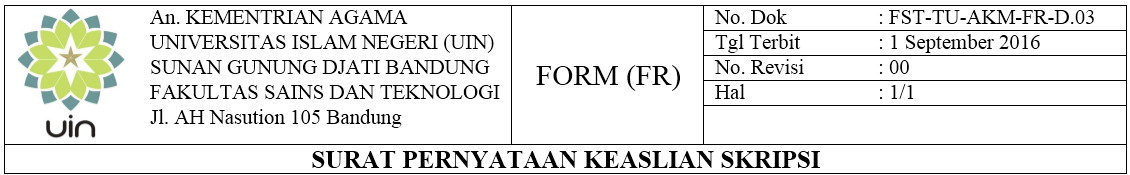
\includegraphics[scale=0.45]{template/head}

\begin{table}
\begin{footnotesize}
\flushright
\begin{tabular}{|c|l|c|l l|}
\hline \hline
&a.n Kementrian Agama&&Nomor Dokumen& FST-TU-AKM-FR-D.03\\\cline{4-5}
&Universitas Islam Negeri (UIN)&&Tanggal Terbit& 1 September 2016\\\cline{4-5}
&Sunan Gunung Djati Bandung&\large{FORM (FR)}&Nomor Revisi& 02\\\cline{4-5}
&Fakultas Sains dan Teknologi&&Halaman& 1/1\\
&Jl. A. H. Nasution 105 Bandung&&&\\\hline
\multicolumn{5}{c}{\bf SURAT PERNYATAAN KEASLIAN SKRIPSI}\cr
\hline
\end{tabular}
\end{footnotesize}
\end{table}

%\chapter*{SURAT PERNYATAAN KEASLIAN SKRIPSI}
 \addcontentsline{toc}{chapter}{SURAT PERNYATAAN KEASLIAN \Model}
\begin{small}
Saya yang bertanda tangan dibawah ini

\vspace{0.3cm}
\begin{tabular}{l l p{15cm}}
Nama &:& \Peneliti \\
NIM &:& \nim \\
Jurusan &:& \Jur \\
\end{tabular} 

\vspace{0.3cm}
Dengan ini menyatakan sebagai berikut :
\begin{enumerate}
\item \model\ yang berjudul \judul\ ini adalah asli dan belum pernah diajukan untuk mendapatkan gelar akademik, baik di \kampus\ maupun di Perguruan Tinggi lain.
\item Karya tulis ini adalah murni gagasan, rumusan, dan penelitian saya, tanpa bantuan pihak lain, kecuali arahan Tim Pembimbing, diskusi teman, dan masukan dari Tim Penelaah.
\item Dalam karya tulis ini tidak terdapat karya atau pendapat yang telah ditulis atau dipublikasikan orang lain, kecuali secara tertulis dengan jelas dicantumkan dalam daftar pustaka sebagai acuan dalam naskah dengan menyebutkan nama pengarangnya.
\item Pernyataan ini saya buat dengan sesungguhnya, apabila di kemudian hari terdapat penyimpangan dan ketidakbenaran dalam pernyataan ini, maka saya bersedia menerima sanksi akademik berupa pencabutan gelar yang telah diperoleh karena karya ini, serta sanksi lainnya sesuai dengan norma yang berlaku di Perguruan Tinggi ini.
\item Lembar pernyataan ini saya buat sebenar-benarnya tanpa ada paksaan dan tekanan dari pihak manapun.
\end{enumerate}
\begin{flushright}
Bandung,\waktu\\
Yang Membuat Pernyataan
\vspace{1.5cm}
\\\Peneliti
\\\nim
\end{flushright}

\end{small}

\chapter*{LEMBAR PERSETUJUAN}  \addcontentsline{toc}{chapter}{LEMBAR PERSETUJUAN}
\begin{center}
\textbf{\Judul} \\
\vspace{0.1cm}
\end{center}
\begin{center}
\textbf{\Peneliti} \\ \vspace{0.1cm}
\textbf{\nim}\\
\end{center}
\begin{center}
\textbf{Menyetujui},\\
\end{center}
\begin{tabular}{c p{3.2cm} c}
Pembimbing 1,& & Pembimbing 2, \\ 
\\
\\
\\
\\
\yudha  &  &  \ridwan \\
NIP. \nipyudha  & & NIP. \\ 
% NIP. \nipyudha  & & NIP. \nipdudung\\
\end{tabular} 
\vspace{0.2cm}
\begin{center}
\textbf{Mengetahui},\\
\end{center}
\begin{tabular}{c p{2cm} c}
Dekan  && Ketua\\
\fak,  &&Jurusan \jur,\\ 
\\
\\
\\
\\
\hasniah  & & \nurul \\ 
NIP. \niphasniah & & NIP. \nipnurul  \\ 
\end{tabular} 
\chapter*{LEMBAR PENGESAHAN}  \addcontentsline{toc}{chapter}{LEMBAR PENGESAHAN}
Skripsi dengan judul : "\textbf{\judul}" telah dipertanggung jawabkan dalam sidang Munaqasyah Jurusan \jur \ \fak \ \kampus \ pada \waktu, dengan majelis yang terdiri dari:

\begin{center}
\begin{tabular}{c p{3.2cm} c}
\\
  & \textbf{Menyetujui} , &\\
Penguji I &  & Penguji II, \\ 
\\
\\
\\
\\
\mada && \imamal\\ 
NIP. \nipmada  & & NIP. \nipimamal\\
\vspace{0.2cm}
\\
  & \textbf{Mengetahui} , &\\
Ketua Majelis,  && Sekretaris, \\
\\
\\
\\
\\
\kaswandhi  && \mada \\ 
NIP. \nipkaswandhi  & & NIP. \nipmada \\ 
\end{tabular} 
\end{center}

%\clearpage
\chapter*{LEMBAR PERSEMBAHAN} \addcontentsline{toc}{chapter}{LEMBAR PERSEMBAHAN}
\vspace{0.5cm}

\begin{center}
\textit{"Allah akan meninggikan orang-orang yang beriman diantaramu dan orang-orang yang diberi ilmu pengetahuan beberapa derajat" (Firman Allah \img{gambar/swt}: Al-Mujadalah,11)}
\vspace{0.7cm}
\\
\textit{"Sesungguhnya, Kami menciptakan segala sesuatu menurut ukuran."(Firman Allah \img{gambar/swt}: Al Qamar,29)}
\vspace{0.7cm}
\\
\textit{"Menuntut ilmu itu diwajibkan bagi setiap muslim dan muslimah."(Sabda Nabi Muhammad \img{gambar/als})}
\vspace{0.7cm}
\\

\end{center}

\begin{flushright}
\vspace{1.5cm}
Ku persembahkan \model\ dalam bentuk \LaTeX\ ini untuk:
\begin{footnotesize}
\\Wawa Wahyudin 
\\Nursilawati
\\Terry Febriani
\\Aldy Rialdy Atmadja
\\Amelia Hasanah 
\\dek Aura
\\dek Zara
\end{footnotesize}
\end{flushright}

%\clearpage


\chapter*{ABSTRAK} \addcontentsline{toc}{chapter}{ABSTRAK}
\begin{tabular}{l l p{10cm}}
Nama &:& \Peneliti\\
Program Studi &:& \jur \\
Judul &:& \judul
\end{tabular} 
\vspace{0.3cm}\\
\vspace{0.1cm}\\

Telah dilakukan penelitian tentang gerak berkelompok yang terdapat pada hewan seperti burung, ikan bahkan manusia. Pergerakan dapat diimplementasikan pada tawaf yang merupakan pola yang yang dipengaruhi oleh keinginan untuk berkelompok agar effisien dan mendekat pada jenis yang sama. keiginan tersebut bergantung pada parameter-parameter tertentu sebagai sistem. Untuk memahami sistem ini dapat dilakukan pendekatan partikel. Interaksi antar partikel dapat digolongkan  sebagai keinginan partikel untuk berkelompok sejenis. dan interaksi kedua dipengaruhi oleh gaya dominan yang memmbuat keinginan tawaf tersebut terpola. Pendekatan Newtonian digunakan untuk
menangani parameter fisika seperti posisi dan kecepatan partikel yang Kemudian dihitung menggunakan integrase runge-kutta. Pola yang muncul diantaranya adalah pola gerak menuju pusat gaya(kaaba). \\

\textbf{\textit{Kata Kunci: gerak berkelompok, runge-kutta, gaya dominan }}

\chapter*{ABSTRACT} \addcontentsline{toc}{chapter}{ABSTRACT}
\begin{tabular}{l l p{10cm}}
\textit{Name} &:& \Peneliti\\
\textit{Studies Program} &:& \prog\\
\textit{Title} &:& \named
\end{tabular} 
\vspace{0.3cm}\\
\vspace{0.1cm}\\

%\textit{Research has been conducted .}\\
Research has been done on group movement found in animals such as birds, fish and even humans. Movement can be applied to tawaf which is a pattern that is influenced by the desire to group together to be efficient and closer to the same type. the desire depends on certain parameters as a system. To understand this system, a particle approach can be used. The interaction between particles can be classified as the desire of particles to group together. and the second interaction is influenced by the dominant force that makes the tawaf desire patterned. The Newtonian approach is used to
handles physical parameters such as position and velocity of the particles which are then calculated using the runge-kutta integration. The patterns that emerge include the pattern of motion towards the center of force (kaaba). \\

\textbf{\textit{Keywords: group movement, runge-kutta, dominant force }}
%%\begin{document}
%\setverb\setnash
%\hyphenpenalty=10000
%\sloppypar
\chapter*{KATA PENGANTAR} \addcontentsline{toc}{chapter}{KATA PENGANTAR}

Segala puji bagi Allah \img{gambar/swt.PNG} \model \ yang berjudul \judul\ dapat diselesaikan. Ini diajukan untuk memenuhi syarat kelulusan program Strata-1 (S1) jurusan \jur, \fak, \kampus. \paragraph{} \model \ ini selesai dengan adanya bantuan dari berbagai pihak. Oleh karena itu penulis ucapkan terima kasih yang kepada: \begin{enumerate} \item Allah \img{gambar/swt.PNG} yang selalu berada di dekat penulis memberikan rahmat dan hidayah untuk menjadi manusia yang berguna.
\item Nabi Muhammad \img{gambar/als.PNG} yang mana beliau adalah panutan bagi penulis.
% \item Bapak DR.Eng.Bagus Endar Nurhandoko, Selaku Direktur Utama PT Rock Fluid Imaging Lab yang telah memberikan kesempatan kepada penulis untuk melaksanakan penelitian Tugas Akhir di Perusahaan PT Rock Fluid Imaging Lab.
% \item Bapak kaswandhi Triyoso.,M.Si dan Bapak Muhammad Rizka Asmara Hadi.,S.T Selaku Dosen Pembimbing Tugas Akhir PT Rock Fluid Imaging Lab, karena atas Bimbingan dan kepercayaan yang beliau berikan kepada penulis untuk menyelesaikan skripsi ini.
% \item Bapak Mada Senjaya W.S., Ph.D Selaku Dosen Pembimbing Jurusan Fisika, karena atas Bimbingan dan kepercayaan yang beliau berikan kepada penulis untuk menyelesaikan skripsi ini.
% \item Bapak Dr.rar.nat. Imamal Mutaqqien.M.Si Selaku Dosen Penguji 1 dan Pembimbing keahlian Fisika Bumi
% \item Bapak Dr.Yudha Setya Perkasa.M.Si, selaku Dosen Penguji 2 dan selaku ketua Jurusan Fisika.    
\item Bapak Dr.Yudha Setya Perkasa.M.Si Sebagai Dosen Pembimbing Akademik Jurusan Fisika, karena atas Bimbingan dan kepercayaan yang beliau berikan kepada penulis untuk menyelesaikan Akademik di Jurusan Fisika  ini.
\item Bapak Ridwan Ramdani, S.Si., M.Si Selaku Dosen Pembimbing Jurusan Fisika, karena atas Bimbingan dan kepercayaan yang beliau berikan kepada penulis untuk menyelesaikan skripsi ini.
\item Seluruh dosen fisika UIN Bandung yang telah banyak meluangkan waktunya untuk memberikan pengetahuan, arahan, masukan, dan dukungan yang berarti bagi penulis. Dan juga senantiasa membimbing penulis mempelajari keilmuan dalam menyelesaikan skripsi ini.
\item Rekan-rekan Fisika angkatan 2015 yang memotivasi  agar penulis lulus sebagai sarjana. 
\item Mahasiswa fisika angkatan 2008, 2009, 2010, 2011, 2012, 2013, 2014 ,2015 ,2016 ,2017 yang selalu memberikan dukungan dan motivasi agar penulis lulus sebagai sarjana.
\item Rekan seperjuangan laboratorium sistem modeling Dinda, Ariq, Arum dan Indri.
% \item Pimpinan dan Keluarga Besar Mahad Tahfidz Al-Quran Al-Kausar 561 Kampung Jagabaya Desa Kecamatan Cineam Kabupaten Tasikmalaya yang telah memberikan tempat penelitian buat penulis untuk melaksanakan penelitian tugas akhir.
% \item Orang tua Bapak H.Yayan Hadian.S.Pd,M.Si dan Ibu Euis Susi Nurhayati.S.Pd.I, adik-adikku Nasiha Al-Sakinah dan Amada Laila Fitria, serta keluarga H.Endang dan H.A Bahrum Sujai yang telah memberikan perhatian, bantuan, motivasi dan pengertian serta doa restu yang penulis sadari mempunyai peran penting dalam menyelesaikan Akademik sehingga penulis lulus sebagai sarjana.
% \item Keluarga kelompok  Desa Sukamatri Kecamatan Tarogong Kaler Kabupaten Garut (KKN) yang pernah bersama-sama hidup selama satu bulan dan memberikan kecerian yang luar biasa. 
\end{enumerate}
\newpage
Akhir kata, penulis menyadari karya tulis ini masih banyak kekurangan oleh karena itu kritik dan saran yang membangun sangat diharapkan demi kesempurnaan skripsi ini. dengan harapan semoga karya tulis ini bermanfaat bagi pembaca khususnya yang mendalami model komputasi.
 
\vspace{0.5cm}
\begin{flushright}
\begin{tabular}{c}
Bandung, \waktu
\\\\\\
Penulis
\end{tabular}
\end{flushright}
%\end{document}
\renewcommand{\contentsname}{DAFTAR ISI}
\tableofcontents \addcontentsline{toc}{chapter}{DAFTAR ISI}
\renewcommand{\listfigurename}{DAFTAR GAMBAR}
\listoffigures \addcontentsline{toc}{chapter}{DAFTAR GAMBAR}
\renewcommand{\listtablename}{DAFTAR TABEL}
\listoftables \addcontentsline{toc}{chapter}{DAFTAR TABEL}
% \renewcommand{\listtablename}{DAFTAR LAMPIRAN}
% \renewcommand{\listtablename}{DAFTAR SINGKATAN}
% \renewcommand{\listtablename}{DAFTAR INDEX}
\chapter*{DAFTAR SINGKATAN}\addcontentsline{toc}{chapter}{DAFTAR SINGKATAN}

\begin{table}
\begin{tabular}{l l l}
% Geoelectric &:& \textit{Geo Electric}\\
% GPS &:& \textit{Global Potitioning System}\\
% Res IP &:& \textit{Resitivity and Induced Polarization}\\
% USB &:& \textit{Universal Serial Bus}\\
FSM : Finite State Machine
HTML : Hyper Text Markup Language\\
CSS : Cascading Style Sheet\\
RAM : Random Access Memory
\end{tabular}
\end{table}

\chapter*{DAFTAR SIMBOL DAN OPERATOR}\addcontentsline{toc}{chapter}{DAFTAR SIMBOL DAN OPERATOR}
\begin{table}
\begin{tabular}{l l l}
$\alpha$	 &:&	Alpha\\
$\upsilon$	 &:&	Kecepatan\\
$p$	 		 &:&	Posisi\\
$m$		     &:&	Massa\\
$t$		 	 &:&	Waktu\\
$\Delta t$	 &:&	Step Size Waktu\\
$\vec{F}$	 &:&	Function Flocking \\
$\sigma$	 &:&	Standard deviasi\\
$\Sigma$	 &:&	Penjumlahan variabel \\
$\pi$		 &:&	nilai pi\\
$e$			 &:&	epsilon\\
$\psi$		 &:&	derajat putaran\\
$\lambda$	 &:&	input state\\
$\kappa$	 &:&	output state\\
$z$			 &:&	radius antar partikel\\




\end{tabular}
\end{table}

%ISI
%\setverb\setnash
%\hyphenpenalty=10000
%\sloppypar
%\begin{document}
\chapter{PENDAHULUAN}\label{cha:pendahuluan}
\pagenumbering{arabic}
%\AddToShipoutPicture{\BackgroundPic}
\section{Latar Belakang}\label{sec:latar}

\hspace{0.6cm} Tawaf merupakan rukun ibadah dalam melaksanakan Haji, dimana seluruh umat islam dianjurkan melaksakannya. Ditinjau dari praktiknya, sederhananya tawaf ialah melakukan pergerakan mengelilingi kaaba sebanyak 7 kali dimulai dari garis hajar aswad dalam satu putaran, ditambah dengan pergerakan menuju hajar aswad dengan sunnah ingin menciumnya.Pergerakan menuju ke hajar aswad menjadikan masalah karena skala yang . Namun sebenarnya dalam keadaan haji, praktik ini menjadi sangat masif karena jumlah variabel individu yang sangat banyak. Penulis mendapatkan cerita, saat melaksanakan praktik ibadah haji, sepasang suami istri sedang melaksanakan salah satu rukun ibadah tawaf mereka sangat ingin mencium hajar aswad, tetapi sangat sulit untuk mencapai inti dari kaaba tersebut, maka mereka bergerak secara berkelompok untuk mencapainya dan berhasil. Fenomena  tersebut sangat menarik karena jika sepasang suami istri tersebut tidak melakukan gerakan berkelompok maka tujuan pusat kaaba tidak tercapai. Sedangkan tawaf merupakan salah satu praktik ibadah yang dilakukan pada saat memasuki Masjidil Al-Haram di Mekkah Saudi Arabi. Tawaf sendiri dilaksanakan pada Umrah dan Haji. Saat Haji, keaadaan tawaf ada di tingkat yang paling tinggi dimana seluruh umat islam berkumpul untuk melaksanakan salah satu pilar islam yang diwajibkan bagi seluruh umat yang mampu. Pada tahun 2017 tercatat sekitar 2.352.122 yang datang dari seluruh dunia untuk melaksanakan haji\citep{Saudi2017}, maka asumsinya seluruh orang tersebut melakukan tawaf bersamaan di waktu yang sama yaitu saat memasuki Masjidil Al-Haram. Jika dibandingkan dengan umrah frekuensi orang yang melakukan tawaf lebih rendah tingkat kepadatan orang. Dan ini menjadikan tawaf, sebagai kegiatan dengan melibatkan jumlah orang terpadat di dunia. Maka merupakan hal yang sulit untuk mencapai pusat kaaba dengan paparan diatas. Menjadikan fenomena ini hal yang menarik untuk dibahas.

% (tulis pergerakan model numerik yang mendukung pemecahan masalah ini)
% Fenomena pergerakan berkelompok inidapat dipetakan melalui berbagai macam m 
\hspace{0.6cm}Fenomena ini dapat diterjemahkan dalam model yang terdiri dari model visual kerumunan dan model teknik numerik yang digunakan. Pertama adalah model visual, karena skalanya yang cenderung besar dengan melibatkan orang banyak. Maka penting untuk mengerti bentuk dari perilaku kerumunan saat melakukan tawaf. Variasi yang dilakukan kerumunan saat berada di Masjidil Al-Haram. Pemahaman terhadap model dari masalah pergerakan kerumunan ini mempunyai solusi berupa sebuah model yang dapat diterapkan, untuk itu diperlukan napak tilas kepada riset tentang perilaku kerumunan. 

\hspace{0.6cm}Riset sebelumnya para ahli dalam bidang kajian aliran kerumunan menggolongkan pada 9 varian major system diantaranya \emph{flocking system}, \emph{behavioral system}, \emph{chaos model system}\citep{Saiwaki1997}, \emph{agent base model}\citep{Khan2012}, \emph{social forces model}\citep{Zainuddin2009}, \emph{hybrid model system}\citep{Shuaibu2015}, \emph{fluid dynamic model}\citep{Narain2009},\emph{cellular automata} \citep{Lim2012}, \emph{cognitive model}\citep{Mulyana2010} and \emph{pedestrian model system}\citep{Adnan2013}. Beberapa studi seperti kim dalam penelitiannya mengguunakan basis kecepatan dan FSM untuk membuat \emph{behaviour system} untuk kerumunan sehingga objek yang berinteraksi dapat mengantisipasi tabrakan dan menghindarinya karena kekuatannya dapat diperhitungkan dari basis kecepatan tersebut\citep{Kim2014}. Studi lainnya deperkenalkan oleh Shuaibu, dengan memodelkan tawaf membentuk jalur spiral menggunakan simulasi \emph{dicrete-event} sistem antri\citep{Shuaibu2015}. Dapat dikatakan ini sebagai model algoritmanya. Dalam riset ini penulis cenderung menggunakan sistem basis agent untuk memodelkan.

\hspace{0.6cm}Kedua adalah tentang model teknik numerik, model numerik ini adalah bagian yang digunakan untuk menghitung sistem dari pergerakan kerumunan ini. 
Dimana hal ini sebagai fondasi dari model untuk variabel dalam model visual. Basis riset untuk teknik numerik ini diantaranya \emph{Finite state machine}\citep{Curtis2011}\citep{Bicho2012},  \emph{Reciprocal Collision Avoidance}, \emph{velocity based model}\citep{Kim2014}, \emph{Ruled Based Model}, Metode Euler dan Langrangian\citep{Narain2009}, \emph{Discrete-event model}.Penulis cenderung menggunakan velocity based model dalam memodelkan sebagai basis fisika interaksinya. %inin harus diterusin dengan referensi
% Salah satu alat untuk menyalurkan ilmu tentang bentuk perilaku orang banyak, dengan memodelkan secara fisis menggunakan komputasi fisis. Bentuk perilaku dapat diterjemahkan kedalam gerak seseorang mengelilingi kaaba saat melakukan tawaf. Waktu tempuh, pola gerak yang terbentuk dalam kepadatan bentuk grup orang yang terbentuk.

Berikut referensi waktu tempuh seseorang untuk menyelesaikan tawaf:
\begin{table}[H]
\begin{tabular}{|c|c|c|c|}
\hline
No.  Sample & Keterangan & Waktu Tempuh(menit) &Sumber Video\\
\hline
1& 3/4 tawaf&	2.14 &matt zimbo banzai\\
\hline
2&full tawaf&	3.07&mustafa aydemir\\
\hline
3&not full circle&	3&-\\
\hline
4&full&	4.2&haris munandar\\
\hline
5&full&	4.32&patarani channel\\
\hline
6&not full&	3/4 tawaf&sukmasari ahmad\\
\hline
7&full&	8.03&best islamic videos\\
\hline
8&full tawaf&	5.05&muhammad raziur rahmad\\

\hline
9&full tawaf&	5.49&stunecity\\

\hline
10&full tawaf&	3.06 umrah& Asep Hendra\\

\hline
11&full tawaf&	4.27&Palmerah Televisi\\

\hline
12&full tawafkhana&	2.2&Najamuddin Shahwani\\

\hline
13&full tawaf&	5.26&All In One Pakistan\\

\hline
14&full tawaf&4.41& I M Zakria\\

\hline
15&full tawaf&	3.44&Samee ur Rahman HSE Trainer\\

\hline
16&full tawaf&	4.48/4.52&Akram Baryar Official\\

\hline 
17&half tawaf&	2.57&HSS pk\\

\hline
18&full tawaf&	4.46&best islamic videos\\

\hline
19&3/4 tawaf&	2.4&Ali Akhtar\\

\hline
20&full tawaf&	3.48&best islamic videos\\

\hline
21&full tawaf&	3.28 bagus& jag Nannn\\

\hline
22&3/4 tawaf&	3.34&My Tech Zone\\
\hline
23&full tawaf&	4.08&bagus akram baryar\\

\hline
24&full tawaf&	-&ikha mabrur pratama\\

\hline
25&3/4 tawaf&	4.24&Panduan Gampang Ibadah \\
& & &Umroh dan Haji  Plus 2014\\
	
\hline
26&1/4 tawaf &	1.15&Muhammad Kahif\\

\hline
27&1/4 tawaf &	1.08&Abdul Waheed kakepoto\\
	
\hline
28&full tawaf&	3.54&	Aryo Pamungkas\\

\hline
29&3/4 tawaf&	3&-\\

\hline
30&7 tawaf&	1=3.01 dan 7=22.47&eljunaed\\
\hline
31&full tawaf&	5.2&Haramain Travels\\

\hline
32&full tawaf&	3.18&Saad Al Qureshi\\
\hline

\end{tabular}
\end{table}

		
\hspace{0.6cm}Pada Riset ini berfokus pada simulasi kerumunan tawaf menggunakan metode flocking dalam pergerakan secara berkelompok. Dengan melakukan variasi \emph{flocking} untuk membentuk pergerakan 1 ras hingga dapat terbentuk sebuah tawaf yang berkelompok sesuai ras pattern partikel. Dengan menggunakan metode runge-kutta. Metode Runge-Kutta ini dipilih karena mempertimbangkan kompleksitas dari metode perhitungan. Jika dibandingkan dengan metode Euler approksimasinya lebih tinggi, dan jika dibandingkan metode newton rapshon lebih rendah aporksimasinya akan tetapi akan menghasilkan kompleksitas perhitungan partikel yang tinggi, akibatnya memperlambat simulasi.
Dalam riset kedepan dapat dikembangkan sebuah metode khusus dalam melaksanakan tawaf yang berbasis struktur dan sistematis. Untuk kedepannya dengan model yang sudah stabil dapat menggambarkan pergerakan tawaf dengan mencapai hajar aswad dengan cara berkelompok   


\section{Rumusan Masalah}\label{sec:rumusan}
Berdasarkan latar belakang yang telah diuraikan maka rumusan masalah dalam penelitian proposal tugas akhir ini adalah sebagai berikut: 

\section{Tujuan Penelitian}\label{sec:tujuan}
\hspace{0.6cm}Tujuan dari penelitian ini adalah membuat sebuah model tawaf mekanisme minimal. Dan menganalisis gaya yang diterapkan agar simulasi stabil antara kelompok tawaf untuk mencapai hajar aswad.

\begin{enumerate}
\item{Bagaimana proses simulasi tawaf bebentuk.}
\item{Bagaimana proses group terbentuk dalam tawaf}
\item{Bagaimana penyederhanaan ruang dan pembatasan individu}
\item{Ruang dalam melakukan tawaf disederhanakan pembatasan individu agar menjaga kestabilan simulasi}
\item{Bagaimana tawaf dapat berkelompok dapat terbentuk dengan tujuan mencapai hajar aswad}
\item{Bagaimana gaya antar kelompok dapat stabil dengan kelompok lain dapat mencapai hajar aswad}
\item{Bagaimana variable yang sudah ditambahkan mempengaruhi simulasi.}
\end{enumerate}

\section{Batasan Masalah}\label{sec:batasan}
Berdasarkan latar belakang yang telah diuraikan maka rumusan masalah dalam penelitian proposal tugas akhir ini adalah sebagai berikut:
\begin{enumerate} 
\item{Semua partikel dianggap sama dan mengikuti aturan yang sama.} 
\item{Berbentuk 2 dimensi.} 
\item{Dibatasi dengan gaya dan perilaku yang telah ditentukan.} 
\item{Bentuk ruang mataf tempat partikel tawaf diserdeharnakan}
\item{Bagaimana proses simulasi tawaf berkelompok  bebentuk.} 
\item{Bagaimana variable yang sudah ditambahkan mempengaruhi simulasi.}
\end{enumerate}


\section{Metode Pengumpulan Data}\label{sec:metode}
\hspace{0.6cm}Dalam penelitian ini digunakan dua metode pengumpulan data yaitu:
\begin{enumerate} 
\item{Studi Literatur}
Sebelum melakukan ekperimen terlebih dahulu dilakukan studi literatur yang dapat bersumber dari berbagai buku, jurnal  dan skripsi untuk mendapat informasi yang dapat dijadikan sebagai acuan selama penelitian.
\item{Metode numerik}
Besaran-besaran pada simulasi akan diupdate menggunakan
metode interasi Runge-Kutta
\item{Simulasi}
Dalam simulasi ini digunakan agent-base model sebagai variable individu yang bergerak secara simulatan dengan variable yang telah ditentukan. Dalam model Masjidil Al-Haram.    

\end{enumerate}


\section{Sistematika Penulisan}\label{sec:sistematika}
\hspace{0.6cm}Pembahasan Pokok dari penelitian ini dibagi menjadi beberapa bab yang diuraikan secara singkat sebagai berikut:

\begin{enumerate}
\item{BAB I PENDAHULUAN
Bab ini menguraikan mengenai latar belakang, perumusan masalah, batasan masalah, tujuan penelitian, metode pengumpulan data, dan sistematika penulisan.}	

\item{BAB II TEORI DASAR
Bab ini berisi teori-teori penunjang penelitian diantaranya agent-base, Behaviour Reciprocal, Reciprocal Collition Avoidance, dll} 

\item{BAB III METODOLOGI PENELITIAN
Pada bab ini diuraikan tahap-tahap dalam penelitian. Tahapan tersebut meliputi: tahap pembacaan data, algoritma program, simulasi perjalanan agent  dalam model yang telah dibentuk.}

\item{BAB IV HASIL SEMENTARA
Pada bab ini akan dibahas tentang hasil sementara penelitian dan analisis yang dibahas dengan acuan dasar teori yang berkaitan dengan penelitian.}

\item{Bab V Kesimpulan dan Saran 
Pada bab ini memuat kesimpulan dan saran yang dapat diambil dari Hasil.
}
\end{enumerate}


%tes \citep{wannamaker04}

%\end{document}%bab 1
%\input{format}
%\begin{document}
%\input{BAB1}
\chapter{TEORI DASAR}\label{cha:teori}
%\AddToShipoutPicture{\BackgroundPic}
%\pagenumbering{arabic}

%%%%%%%%%%%%%%%%%%%%%%%%%%%%%%%%%%%%%%%%%%%%%%%%%%%%%%%%%%%%%%%

\section{Model Interaksi}\label{sec:modelinteraksi}
\hspace {0.5cm}Dalam melaksanakan tawaf gerak individu dapat dikaitkan dengan perilaku interaksi individual, karena bentuk kecepatan pergerakan orang pertama dalam melaksanakan tawaf bergantung dengan orang kedua didepannya dan orang didepannya tergantung dengan orang ketiga didepannya lagi dan seterusnya. Kita dapat meninjaunya dari segi fisika dengan mengasumsikan setiap individu adalah partikel. Partikel bergerak berkelompok karena kecepatan tetap dan arah setiap partikel resultan dari semua partikel berkelompok tersebut.

\hspace {0.5cm}Proses resultan dari partikel gerak individual menuju partikel yang berkelompok diakibatkan oleh perubahan variabel dalam sistem gaya yang mempengaruh.Variabel yang digunakan tersebut terletak pada order parameter. Orde parameter ini yang diterapkan kedalam mekanika \textit{flocking} .

\hspace {0.5cm}Dalam flocking yang dijalankan, terdapat \textit{input state} dan \textit{output state} yang digunakan dalam proses properti model partikel . Properti partikel ini berbentuk posisi, kecepatan, massa dan jarak gaya yang akan ditinjau dalam simulasi. Properti ini dalam \citep{Bajec2007} disebut dengan \textit{current state properties}  $q$. Yang dimaksud \textit{current state properties} adalah karakteristik yang dimiliki setiap partikel.
\begin{equation}
q = {p,\upsilon,z,m,\psi} 
\end{equation}



\section{Aplikasi gaya}\label{cha:aplikasi gaya}
\subsection{Flocking}\label{sec:flocking}

Mekanika Flocking berdasarkan reynolds mempunyai 3 gaya yang digunakan untuk membentuk kerumunan   \citep{Reynolds1987} \citep{Nasir2016}. Dimana hal ini dipakai oleh \citep{Chate2008} dalam modelnya \emph{boids model} untuk simulasi. Simulasi kerumunan akan terbentuk jika partikel bergerak sama dengan partikel sekitarnya, ,membentuk 1 titik area pemadatan partikel, dan mempunyai gaya pemisah agar partikel bergerak tanpa adanya partikel yang melekat/ tumbukan tidak elastis. Interaksi antar kerumunan ini dalam \citep{Chate2008} dinamakan SPP(\texttit{Self-Propelled Particles}). 

\begin{equation}
\vec{F}_i = \sum_{i \neq j} (\sum_{n=1}^{\infty} R_{n} \dfrac{\vec{P}_{ij}}{|\vec{P}_{ij}|^n}  + \sum_{n=1}^{\infty} I_{n} \dfrac{\vec{P}_{ij}}{|\vec{P}_{ij}|^n}). 
\end{equation}

\subsubsection{Alignment}\label{sec:alignment}
\hspace {0.5cm} Gaya Allignment digunakan untuk membuat partikel tetap bergerak satu grup. Berkaitan dengan sistem dalam tawaf, digunakan karena di dalam masjidil haram beberapa orang sering berkerumun untuk membentuk 1 grup agar tidak tersesat. Alasan lainnya, untuk penggunaan alignment ini membuat partikel menyamakan persepsi kecepatan dengan konsep yang terdepan akan mengurangi kecepatannya juga yang belakang akan menambah kecepatannya untuk berjalan bersamaan membentuk grup. secara matematika dapat ditulis sebagai berikut.

\begin{equation}
 F_i^a(p,q) = \alpha^a \dfrac{1}{N^c}\sum^{N^c}_{i \neq j}\dfrac{\vec{V}_{ji}}{|\vec{V}_{ji}|},\alpha^a = 1N
\end{equation}


\begin{figure}
\centering
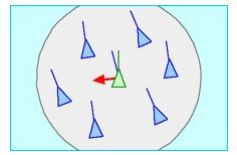
\includegraphics[scale=0.5]{gambar/allignment}
\caption{Bentuk Gerak Pensejajaran}
\end{figure}

\subsubsection{Cohesion}\label{sec:cohesion}
\hspace{0.5cm}Gaya kohesi digunakan untuk membuat partikel menarik tetangganya untuk berdekatan. Dimana posisi pusat dijadikan titik arah pergerakan sehingga partikel bergerak ke titik tersebut: berikut secara matematik dapat ditulis:

\begin{equation}
 F_i^k(p,q) = \alpha^k \dfrac{1}{N^c}\sum^{N^c}_{i \neq j}\dfrac{\vec{p}_{ji}}{|\vec{p}_{ji}|} , \alpha^k = 1N
\end{equation}
\begin{figure}
\centering
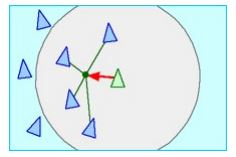
\includegraphics[scale=0.5]{gambar/cohesion}
\caption{Bentuk Gerak Pemusatan}
\end{figure}

\subsubsection{Separation}\label{sec:separation}
\hspace{0.5cm} Gaya separasi digunakan untuk partikel agar terjadi pemisahan dan meminimalisir pemisahan. Dalam konteks tawaf digunakan untuk menghindari seseorang menempal terhadap orang lain. dalam gaya separasi ini dilakukan variasi terhadap koefisiennya yaitu koefisien introversion atau tingkatjaga jarak dan tingkat racis untuk mengelompokkan jenis ras partikel berdasarkan warna.

\begin{equation}
 F_i^s(p,q) = \alpha^s \sum^{N^c}_{i \neq j}\dfrac{\vec{p}_{ji}}{|\vec{p}_{ji}|^2},\\
 \end{equation}
\begin{equation}
\alpha^a = radius + radius boids tetangga + koefisien introversion + koefisien racism
 \end{equation}

\begin{figure}
\centering
\includegraphics[scale=0.5]{gambar/separation}
\caption{Bentuk Gerak Pemisahan}
\end{figure}

\subsubsection{Circular Motion}\label{sec:circularmotion}
\hspace{0.5cm}Circular Motion atau bisa disebut gaya gerak memutar mengelilingi pusat gaya, dapat diaplikasikan kepada partikel yang bergerak secara flocking untuk membuat partikel seperti bergerak tawaf mengelilingi pusat gaya. Dimana pusat gaya berada di pusat kaaba berbentuk persegi. Gerak Flocking yang diterapkan perlu memenuhi syarat area tawaf. Dengan begitu gerak mengeliligi kaaba dapat berada di area dekat kaaba.

\[
  f(x)=\begin{cases}
    F_m^a(p,q) = \alpha^m \sum^{N^c}_{i \neq j}\dfrac{\vec{p}_{ji}}{|\vec{p}_{ji}|},\alpha^m = 1N , & \text{if x<50}.\\
    F_m^a(p,q) = \alpha^m \sum^{N^c}_{i \neq j}\dfrac{\vec{p}_{ji}}{|\vec{p}_{ji}|},\alpha^m = -1N, & \text{if x>50 and if x>300 }.
  \end{cases}
\]

\hspace{0.5cm}Pada persamaan pertama penerapan gaya menjauhi kaaba dengan syarat angka 50 jarak dari pusat kaaba sampai dinding. Sedangkan pada persamaan kedua penerapan gaya mendekati kaaba dengan asumsi partikel berada di luar area 50 sampai 300. Kedua gaya ini adalah gaya dominan yang diterapkan agar circular Motionnya bekerja.


\hspace{0.5cm}Penerapan gaya terbagi dalam 3 area,yaitu area dibagian luar putar,area dimana tawaf diterapkan dan area dinding kaaba. Pada bagian luar diterapkan gaya tarik menuju pusat, dibagian diding kaaba diterapkan gaya keluar untuk menjaga dinding kaaba. di area diterapkan gaya putar untuk partikel melakukan tawaf.


%%%%%%%%%%%%%%%%%%%%%%%%%%%%%%%%%%%%%%%%%%%%%%%%%%%%%%%%%%%%

\section{Model Partikel}\label{sec:modelpartikel}
\hspace {0.5cm}Model partikel sederhana dengan bentuk bulat menggambarkan partikel agent yang sedang bergerak
\begin{figure}
\centering

\includegraphics[scale=0.3]{gambar/ModelPartikel.JPG}
\caption{Model partikel sebagai titik posisi}
\end{figure}


\section{Model Ruang Partikel}\label{sec:ruangpartikel}

\hspace {0.5cm}Model ruang Partikel diformulasikan seperti gambar masjidil haram yang tertera pada gambar. Partikel bergerak berlawanan arah dengan ruang dibatasi boundary state yaitu dinding masjidil haram dan bagian dalam ada boundary state lagi berupa dinding kaaba. Akan tetapi dalam simulasi ini model ruang partikel dibatasi hanya pada kaaba dan area tawaf kaaba.
\begin{figure}
\centering
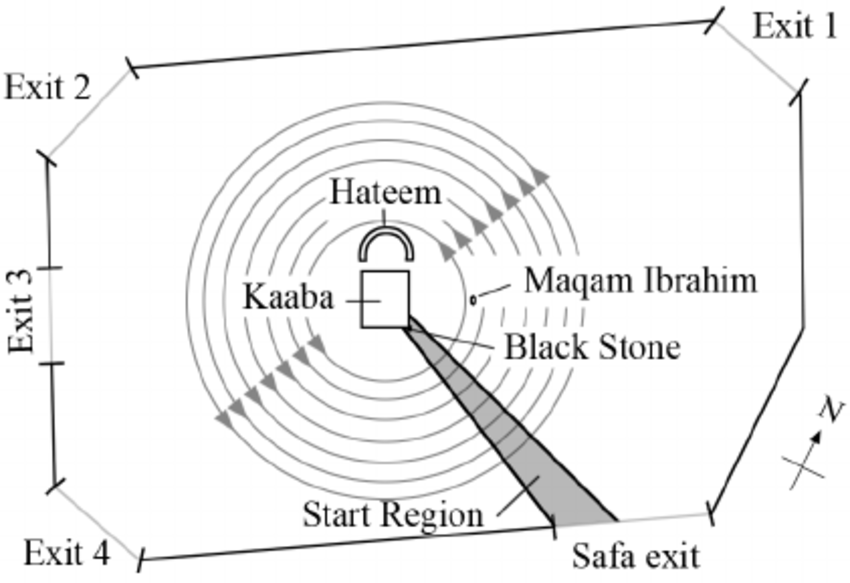
\includegraphics[scale=0.5]{gambar/layout2dmasjidilharam}
\caption{Model Area Masjidil Haram}
\end{figure}

\section{Persamaan Distribusi Normal }\label{sec:modelpartikel}
\hspace{0.5cm} Distribusi normal dalam program ini digunakan untuk menentukan nilai real dari koeffisien yang ada dalam nilai introversi, rasisme dan ketangkasan(quirkness). Hal ini mempengaruhi bentuk dari inisial tawaf yang akan terjadi, dalam kasus ini secara acak. 

\begin{equation}
f(x) =\dfrac{1}{\sigma \sqrt{2 \pi}} e^{-\dfrac{1}{2}(\dfrac{x-\mu}{\sigma})^2}
\end{equation}

\hspace{0.5cm} Normal distribusi penting digunakan dalam statistik karena sering digunakan untuk representasi nilai real dari variabel random yang distribusinya tidak diketahui\citep{Caseberg2009}. Pada simulasi ini distribusi normal digunaakan sebagai perbandingan untuk koefisien  partikel  agar dapat divariasikan.





\section{Metode Runge Kutta}\label{sec:metodeperhitungan}
\hspace{0.5cm} Metode Runge-Kutta adalah metode numerik yang banyak digunakan untuk menyelesaikan persamaan differensial. Metode ini adalah versi yang lebih kompleks dari metode euler yang banyak digunakan. Karena kompleksitasnya maka metode ini menawarkan grafik eksponensial yang lebih mendekati fungsi eksak.\\
Untuk fungsi y
\begin{equation}
\dfrac{dy}{dt} =f(y,t) , y(t_0)=y_0
\end{equation}

\begin{equation}
y_{n+1} = y_{n} + \dfrac{1}{6}h (k_1+2k_2+2k_3+k_4),
\end{equation}

\begin{equation}
Untuk n = 0,1,2,3,4 ......\\
\end{equation}
\begin{equation}
k_1 = f(y_{n} ,t_{n}),\\
\end{equation}
\begin{equation}
k_2 = f(y_{n}+h\dfrac{k_1}{2} ,t_{n}+\dfrac{h}{2}),\\
\end{equation}
\begin{equation}
k_3 = f(y_{n}+h\dfrac{k_2}{2} ,t_{n}+\dfrac{h}{2}),\\
\end{equation}
\begin{equation}
k_4 = f(y_{n}+hk_{1} ,t_{n}+h).\\
\end{equation}
\\
Untuk fungsi x
\begin{equation}
\dfrac{dx}{dt} =f(x,t) , x(t_0)=x_0
\end{equation}

\begin{equation}
x_{n+1} = x_{n} + \dfrac{1}{6}h (k_1+2k_2+2k_3+k_4),
\end{equation}

\begin{equation}
Untuk n = 0,1,2,3,4 ......
\end{equation}
\begin{equation}
k_1 = f(x_{n} ,t_{n}),
\end{equation}

\begin{equation}
k_2 = f(x_{n}+h\dfrac{k_1}{2} ,t_{n}+\dfrac{h}{2}),
\end{equation}

\begin{equation}
k_3 = f(x_{n}+h\dfrac{k_2}{2} ,t_{n}+\dfrac{h}{2}),
\end{equation}
\begin{equation}
k_4 = f(x_{n}+hk_{1} ,t_{n}+h).
\end{equation}


\begin{figure}

\centering
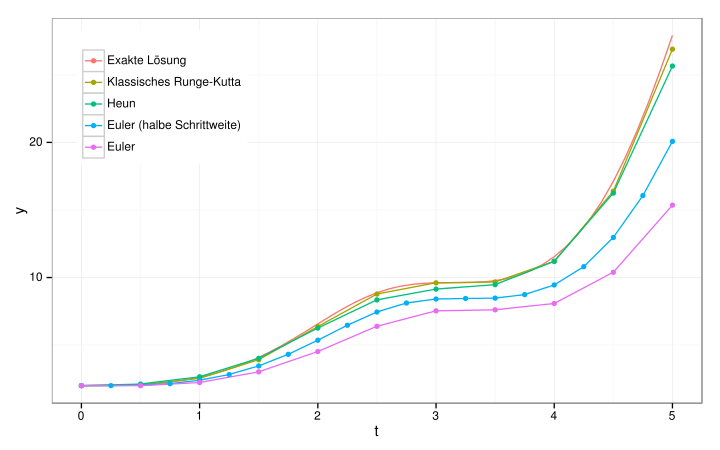
\includegraphics[scale=0.5]{gambar/comparison_euler}
\caption{Perbandingan euler dan runge-kutta}
\end{figure}

Dalam simulasi ini penggunaan runge-kutta digunakan karena alokasi memori komputer yang digunakan tidak terlalu besar. Metode ini juga dipertimbangkan dengan metode euler dimana tingkat error yang lebih rendah. Mempertimbangkan jumlah partikel yang digunakan maka diambil metode ini. Metode runge-kutta digunakan karena kinerja pada komputer ringan.



%\input{referensi}
%\end{document}%bab 2
%\setverb\setnash
%\hyphenpenalty=10000
%\sloppypar
%\begin{document}
\chapter{METODOLOGI PENELITIAN}\label{cha:metodologi}
%\pagenumbering{arabic}
%\AddToShipoutPicture{\BackgroundPic}
%\DeclareUnicodeCharacter{FFFD}{?????}
\section{Alat yang Digunakan}\label{sec:alat}
\subsection{Perangkat Keras}\label{sec:perangkatk}
\hspace{0.6cm}Perangkat keras yang digunakan adalah sebuah laptop dengan spesifikasi sebagai
berikut:

\begin{table}
\centering
\caption{Spesifikasi Perangkat Keras.}
\begin{center}
\begin{tabular}{|c|c|c|}
\hline
No & Komponen & Spesifikasi \\
\hline
1 & Processor & Intel(R) Core(TM) i5-4300M CPU @ 2.60GHz 2.59 \\
\hline
2 & Memory & 12GB \\
\hline
3 & Display & Intel(R) HD Graphics 4600 \\
\hline
4 & Renderer & - \\
\hline
5 & OS & Windows 10 \\
\hline
\end{tabular}
\end{center}
\end{table}

\subsection{Perangkat Lunak}\label{sec:perangkatl}
\hspace{0.6cm}Perangkat lunak yang digunakan :

\begin{table}
\centering
\caption{Spesifikasi Perangkat Lunak.}
\begin{center}
\begin{tabular}{|c|c|c|}
\hline
No & Komponen & Software \\
\hline
1 & Text Editor & Sublime \\
\hline
2 & Browser & Google Chrome \\
\hline
3 & Library & victor js library \\
\hline
\end{tabular}
\end{center}
\end{table}

\hspace{0.6cm}Perangkat keras pada Tabel 3.1 adalah milik pribadi penulis. Meninjau simulasi
akan menggambar banyak partikel yang dihitung terus menerus maka graphic card dan RAM yang digunakan sebaiknya tidak jauh berbeda dengan yang dimiliki
penulis. Adapun perangkat lunak pada Tabel 3.2 yang digunakan dapat ditemukan
secara gratis di internet



\section{Penerapan Gaya}

\subsection{Penerapan 3 gaya}
\hspace{0.6cm}Pola flocking dimana partikel diproyeksikan bergerak membentuk formasi berkelompok sesuai dengan groupnya.Untuk hal tersebut diterapkan partikel disimulasikan dalam kasus dimana partikel dimunculkan pada tempat yang acak. setelahnya partikel akan bergerak dipengaruhi 3 gaya yaitu alignment, cohesion, dan separation. Sampai pola gerak berkelompok terbentuk

\subsection{Penerapan 3 gaya ditambah gaya circular}

\begin{equation}
\vec{F}_i = \vec{F^a}_i + \vec{F^k}_i + \vec{F^s}_i + \vec{F^c}_i
\end{equation}

\hspace{0.6cm}Pada kasus dengan tambahan gaya circular, partikel akan diterapkan gaya pusat circular sebagai prioritas agar partikel bergerak didalam area tawaf. dan ketika berada diarea tawaf partikel bergerak secara circular berlawanan arah jarum jam. dalam area tawaf ada gaya yang sama untuk mencegah agar partikel tetap berada di area tawaf.
untuk prioritas gaya maka ada massa factor (m) sebagai besar factor prioritasnya.

\begin{equation}
\vec{F}_i = m^a\vec{F^a}_i + m^k\vec{F^k}_i + m^s\vec{F^s}_i + m^c\vec{F^c}_i
\end{equation}

\subsubsection{interaksi diluar zona tawaf}
\hspace{0.6cm} Maksud dari interaksi diluar tawaf. adalah partikel hanya bergerak menuju ke zona tawaf. Dengan gaya partikel lain yang minim. Hal ini menggiring partikel menuju pergerakan di area tawaf.

\subsubsection{interaksi didalam zona tawaf}
\hspace{0.6cm} Pada kasus ini partikel berinteraksi dengan group partikel lain, juga berinteraksi dengan partikel yang berbeda group juga. Partikel dengan group sama diwakilkan dengan warna yang sama mempunyai gaya separasi yang lebih kecil dibandingkan dengan partikel yang berbeda groupnya. 

Adapun gaya circular dalam simulasi digunakan untuk partikel melakukan putaran tawaf. Flocking juga dapat distabilkan jika kelompok partikel berkumpul dengan sejenisnya, Membentuk group sambil melakukan tawaf. Hal ini mencerminkan partikel menjaga eksistensi groupnya, sambil melakukan tawaf.

\section{Simulasi Komputer}
\hspace{0.6cm}Simulasi dan program dibagun dalam bahasa JavaScript sebagai dasar codenya. secara visual menampikan animasi dan grafik yang menghasilkan outputnya.Bentuk matematis program dimuat dalam library Victorjs. Dimana fungsi kalkulasi vektor terdapat dalamnya, sehingga dapat dipanggil dengan mudah.

\begin{table}
\centering
\caption{Sekilas tentang pengunaan library VictorJS .}
\begin{center}
\begin{tabular}{|c|c|}
\hline
Penulisan koordinat  & Penulisan koordinat\\
gaya menggunakan victorjs &  gaya tanpa victor js menggunakan array javascript\\
\hline
var Vector = new Victor(diff.x,diff.y); & var Vector = [diff.y,diff.y] \\
\hline
\hline
sum.add(Vector) & Vector = [diff.y,diff.y] + [sum.y,sum.y]  \\
\hline
\end{tabular}
\end{center}
\end{table}

\hspace{0.6cm}Tabel diatas menggambarkan penulisan Koordinat menggunakan \emph{library} Victor.js\citep{noauthororeditor2014victorjs}. Gaya berbentuk array dalam program biasa dapat dikonversi kedalam \emph{library} menggunakan victor.js, di dalam victor.js juga terdapat perintah untuk menjumlahkan gaya dengan singkat seperti terdapat pada no 2. Terdapat banyak lagi selain penjumlahan vector, pengurangan, akar kuadrat dan lain-lain.  



\begin{figure}
\centering
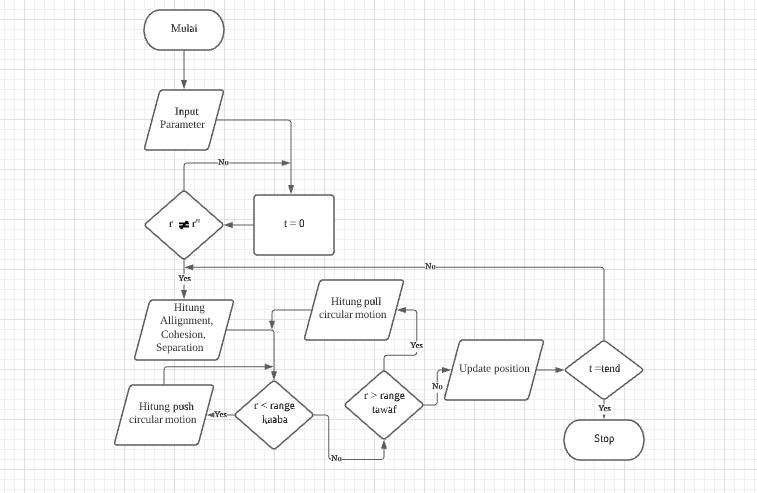
\includegraphics[scale=0.5]{gambar/diagram} %gambarnya harus algoritma
\caption{Algoritma Pemograman.}
\end{figure}

\section{Parameter Gaya}
% Parameter gaya dijabarkan pada bab 2 diantaranya
\subsection{Parameter dalam pergerakan gaya}
\hspace{0.6cm}Dalam penerapannya, hasil simulasi kaaba diletakan di pusat dengan titik (sekian) dimana parameter penting lainnya adalah koordinat partikel yang dimunculkan secara acak dalam ruang interaksi zona tawaf maupun zona diluar tawaf. Partikel juga memiliki sebuah id untuk mengkatagorikan partikel dalam sebuah kelompok. Parameter selajutnya adalah gaya antar partikel yang diatur agar partikel membuat sebuah group, dalam hal ini, gaya separasi yang (koefisien \emph{boid} < koefisien partikel lain) akan membuat partikel memilih jarak yang yang berbeda sesuai dengan group partikelnya. parameter lain yang berpengaruh adalah gaya tarik kedalam zona tawaf agar partikel membuat gerakan tawaf. Jumlah partikel N ditentukan untuk menguji kestabilan simulasi dalam hal ini dibatasi dengan jumlah orde 3 digit untuk menghindari adanya laging dalam proses simulasinya.

Dalam \emph{interface}, gaya separasi dibentuk dari salah satu variabel yaitu jarak separasi($z_s$) didalamnya dalam  terdapat koefisien introversi dan koefisien rasis dimana koefisien ini membentuk radius maksimum untuk melakukan gaya separasi dimana desiredSeparation = radius boid + radius boid lain + ( 25 * koefisien introversion ) + ( 50 * racismMultiplier koefisien ). Pada koefisien racism diterapkan logika bahwa jika partikel memiliki warna sama maka koefisien racism akan menjadi nol, dan jika tidak maka akan mempunyai nilai. Nilai ini yang mengaktifkan gaya separasi.

Parameter lain yang mempengaruhi gaya adalah jarak pensejajaran $z_a$, dimana ada aturan jarak yang dibutuhkan untuk gaya mempengaruhi boid agar melakukan pensejajaran dengan \emph{boid} lain parameter jarak ini adalah 25.

Parameter lain yang mempengaruhi gaya adalah jarak kohesi$z_k$, dimana ada aturan jarak yang dibutuhkan untuk gaya mempengaruhi boid agar melakukan kompresi dengan boid lain parameter jarak ini adalah 25.
\subsection{Parameter variasi partikel yang ditambahkan dalam simulasi}
Pada simulasi ditambahkan partikel dengan speed yang berbeda. Terdapat 3 variasi kecepatan yang digunakan diantaranyaa quickness = 1 ,agroQuickness = 1.25 dan blackQuickness = 0.5. Pada partikel yang merah ditentukan parameter kecepatan yang 1.25 koefisien dari kecepatan normal. Pada partikell hitam ditentukan koefisien nya yaitu 0.45 dari kecepatan normal.
% \subsection{Perhitungan koefisien introversion dan rasisme}
% \hspace{0.6cm}untuk mendapatkan nilai koefisien yang diperlukan gaya diperlukan nilai distribusi normal untuk menjaga sebuah koefisien setiap simulasi dijalankan berbeda tetapi tidak membuat simulasi tidak stabil.

% dengan persamaan 2.6 kalkulasi koefisien dari introversion and rasisme dapat dikalkulasikan, nilai dari variabel mean adalah 50 dan standard deviasinya adalah 9.


%tes \citep{wannamaker04}

%\end{document}%bab 3
%\input{format}
%\begin{document}
%\input{BAB1}
%\input{BAB2}
%\input{BAB3}
\chapter{Hasil dan Pembahasan}\label{cha:Hasil}



\section{Flocking tanpa Circular Motion}%\label{sec:alat}
% \begin{figure}
% \centering
% 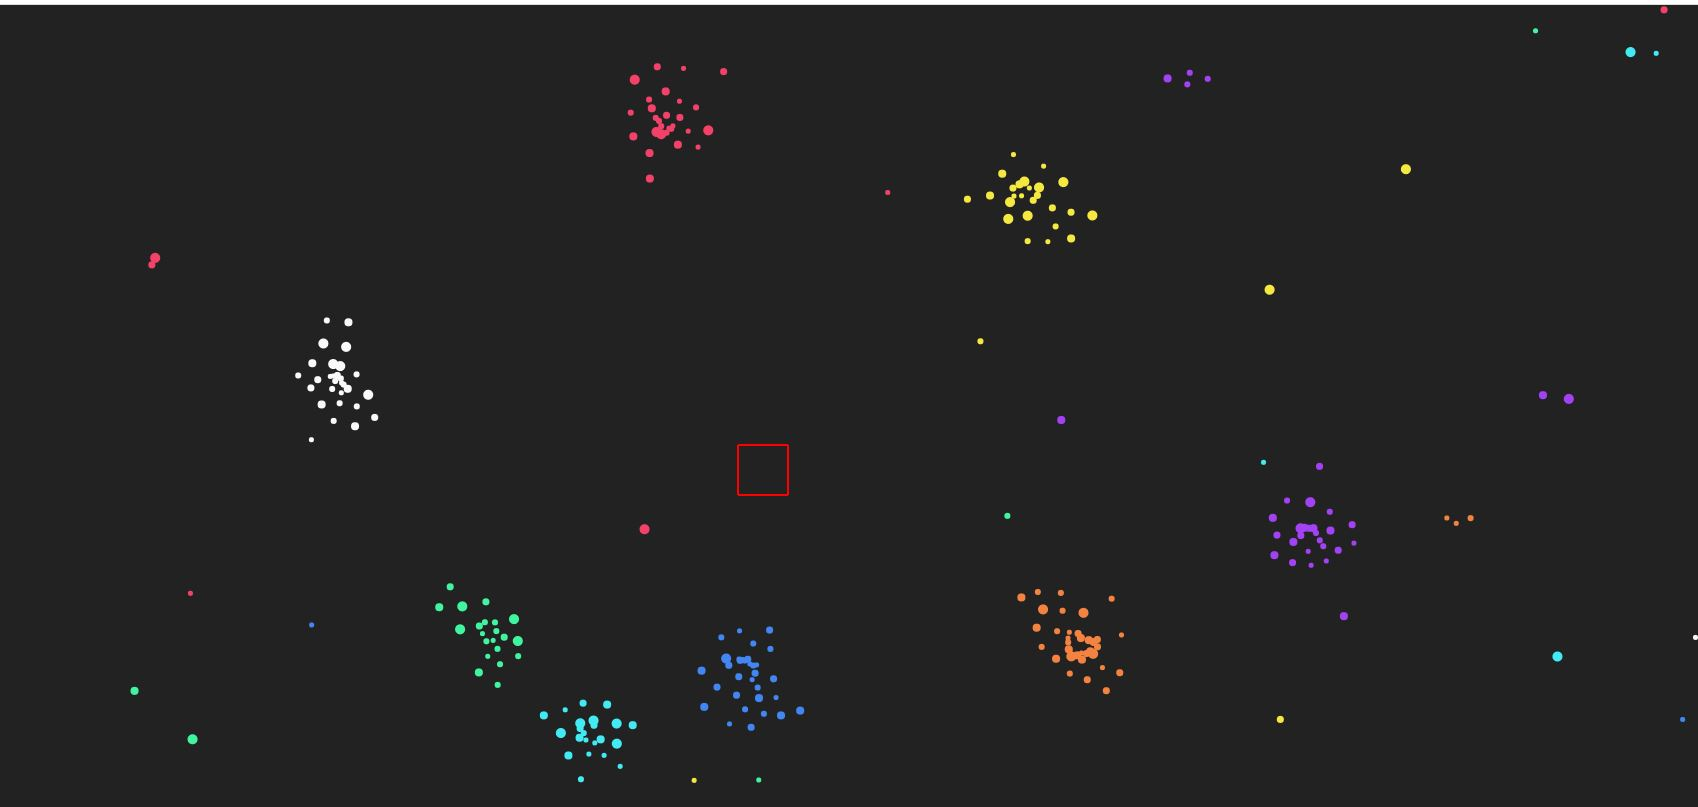
\includegraphics[scale=0.4]{gambar/example}
% \caption{Hasil Model alligment,separation dan kohesi}
% \end{figure}
% \hspace{0.6cm}
\begin{figure}
\centering
\subfigure[Model Flocking dengan range 25 N=100]{\label{fig:flocking dengan range 25}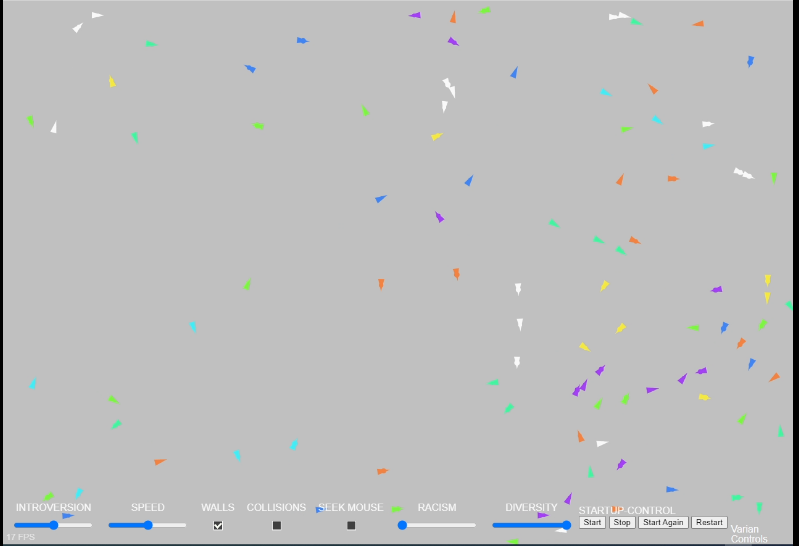
\includegraphics[scale=0.3]{gambar/gambar1notawafflocking25}}

\subfigure[Grafik Model Flocking dengan range 25 N=100]{\label{fig:grafik flocking dengan range 25}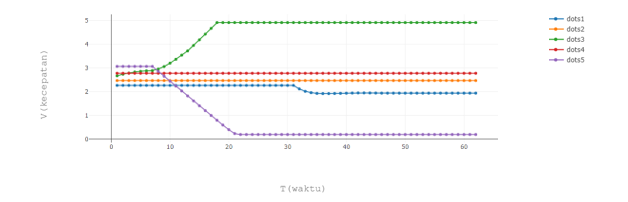
\includegraphics[scale=0.3]{gambar/datagrafik/range25homogennoflocking}}

\subfigure[Model Flocking dengan range 50 N=100]{\label{fig:flocking dengan range 50}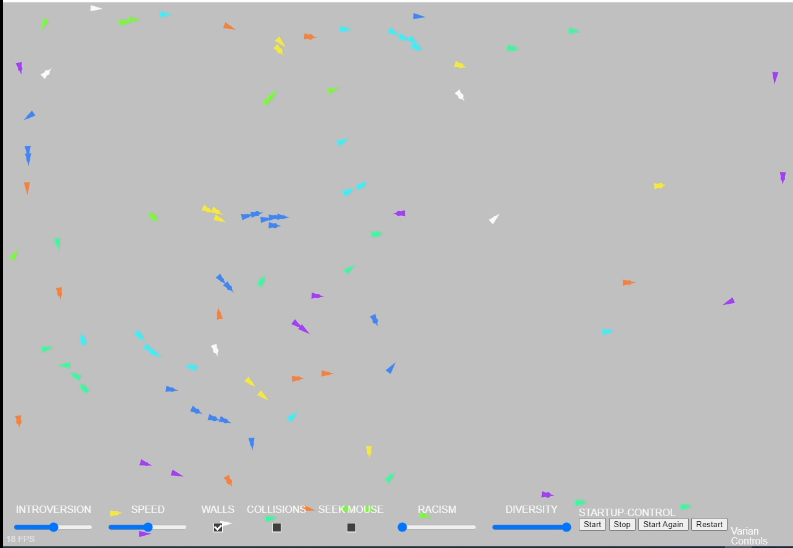
\includegraphics[scale=0.3]{gambar/gambar2notawafflocking50}}

\subfigure[Grafik Model Flocking dengan range 50 N=100]{\label{fig:grafik flocking dengan range 50}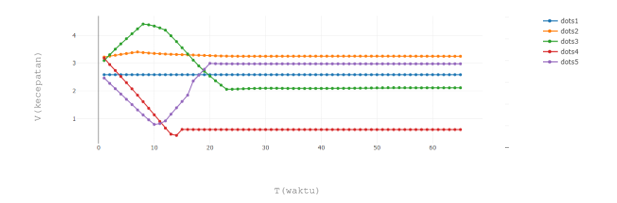
\includegraphics[scale=0.3]{gambar/datagrafik/range50noflocking}}

\caption{Hasil Model alligment,separation dan kohesi dengan range 25 dan range 50}
\label{fig:2grafikmodel3gaya}
\end{figure}

% Pada hasil ini formasi partikel terlihat bisa membedakan partikel hal ini karena 
Hasil pada model flocking tanpa gerakan tawaf(\textit{circular motion}) dengan range \textit{flocking} yang berbeda pada kohesi dan pensejajarannnya, dapat dibandingkan kedua pengoptimalan range dalam menentukan pergerakan partikel . Hal ini dapat dibandingkan dengan \citep{HUTH1992} juga yang membuat \textit{range}, agar perbedaan pergerakan partikel dapat terlihat.Pada gambar \ref{fig:2grafikmodel3gaya} partikel yang mempunyai \textit{range} 50 cenderung lebih mudah berkelompok  dari pada range 25. hal ini wajar karena semakin besar range dalam \textit{flocking} yang digunakan maka semakin mudah dalam partikel berkelompok. Pada partikel dengan range 50 berkelompok adalah 4 partikel 
sedangkan pada partikel dengan range 25 rata2 berkelompok adalah 2 partikel.
% \hspace{0.6cm}Hasil sementara berupa gerak flocking yaitu allignment, separation dan kohesion yang dipadukan dengan fungsi mencari titik pusat. Metode yang digunakan masih euler karena memperhitungkan buffer yang terjadi jika memakai runge kutta.  Koeffisien separation divariasikan dengan racism dan introversion agar terlihat jamaah mempunyai identitas yang berbeda. Pembentukan formasi berdasarkan warna partikel dimana partikel mampu membedakan satu sama lain 

%%%%%%%%%%%%%%%%%%%%%%%%%%%%%%%%%%%%%%%%%%%%%%%%
\section{Flocking dengan Gaya Dominan(Circular Motion)}%\label{sec:alat}

\begin{figure}
\centering
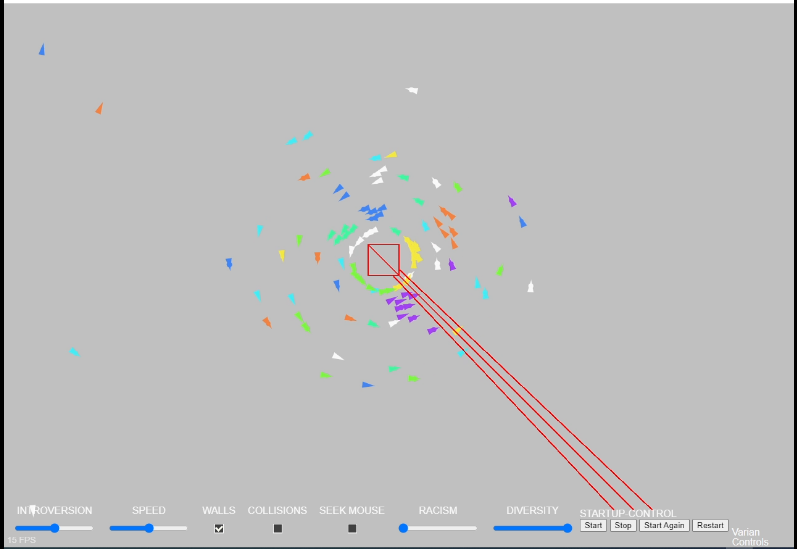
\includegraphics[scale=0.6]{gambar/gambar3tawafflocking25}
\caption{Hasil Model dengan ditambahkan gaya dominan, N=100}
\label{fig:2grafikmodel4gayadengan dominanforce}
\end{figure}
\hspace{0.6cm} Pada bagian ini ditambahkannya gaya dominan pada persamaan 2.5 dimana gaya dominan ini berfungsi mengikat partikel untuk berputar pada porosnya.Terdapat perbedaan antara pergerakan tanpa circular motion adalah flocking hanya bekerja pada area tawaf. Dan partikel diluar area tersebut akan perlahan mendekati area tawaf. Hal ini dilakukan untuk mendekati \citep{Nasir2016} dan \citep{Kim2014}. Dimana apa yang dilakukan nasir adalah mengelompokan agent(partikel) dalam sebuah group dikelilingi partikel yang homogen. sedangkan pada \citep{Kim2014} mengamplikasikan flocking ditambahkan dengan reciprocal coalition avoidance. untuk memperlihatkan interaksi partikel yang lebih tidak bersinggungan. Jika dapat dianalisis hasil pada \ref{fig:2grafikmodel4gayadengan dominanforce} didapat konsep \citep{Nasir2016} yang menggolongkan partikel dan konsep dari \citep{Kim2014} untuk flocking berbasis kecepatan.
\begin{figure}
\centering
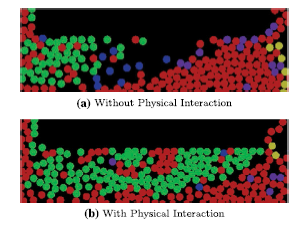
\includegraphics[scale=0.6]{gambar/Kim2014}
\caption{hasil gerak partikel pada \citep{Kim2014}}
\label{fig:figkim2014}
\end{figure}
% Pushed by crowd. Green circles represent the agents in the
% queue waiting to touch the black stone. The green agents slow down and
% the result in heavy congestion at the beginning of the queue. Without
% physical interactions, agents are stuck in the beginning of the queue
% although there is a space in front of the queue to proceed. By adding
% physical interactions, the agents in the queue are pushed by the crowds,
% and move towards the black stone without breaking the queue.

% Due to the sudden slowdown caused by the green agents,
% heavy congestion is made at the beginning of the queue.Without adding physical interactions, we cannot capture the effect
% of crowd force applied to these agents even in such high density. Agents are stuck in the beginning of the queue although
% there is a space in front of the queue to proceed. By adding
% physical interactions, the agents in the queue are pushed by
% the crowds, and move towards the black stone without breaking the queue.
\hspace{0.6cm} Pada gambar \ref{fig:figkim2014} diperlihatkan hasil kim bahwa partikel (agen) terpadatkan di dekat pusat area gaya(kaaba). Hal ini dikarenakan terdorong oleh kerumunan agen. Pada gambar agen hijau menunjukan agen yang menunggu menyentuh titik pusat gaya(hajar aswad). Diawal simulasi agent berada dalam keadaan tidak dapat bergerak dan menghasilkan kerumunan padat. Tanpa interaksi fisis meskipun ada ruang gerak, partikel agent tidak bisa memproses ke posisi selanjutnya. Denggan tambahan interaksi fisis dengan agent selanjutnya agent dapat terdorong oleh kerumunan.
% \hspace{0.6cm}Dapat terlihat bentuk tawaf telah terbentuk, mungkin harus ada adjustment gaya lagi supaya geraknya selalu melawan arah jarum jam. Boundary state untuk partikel juga belum diterapkan seperti dinding kaaba dan outer dinding bagian masjid, kemunculan partikel sendiri harus ada adjustment. dan harus ada adjustment lagi tentang layar yang digunakan untuk menetukan kecepatan yang terbentuk.
%%%%%%%%%%%%%%%%%%%%%%%%%%%%%%%%%%%%%%%%%%%%%%%%
\section{Flocking dengan Gaya Dominan(Circular Motion) partikel dengan Karakteristik}%\label{sec:alat}

% \begin{figure}
% \centering
% \includegraphics[scale=0.4]{gambar/}
% \caption{Hasil Model Sementara}
% \end{figure}
\begin{figure}
\centering
\subfigure[Model Flocking dengan range 25 N=100 gaya dominan tawaf]{\label{fig:flocking dengan range 25 dominan force}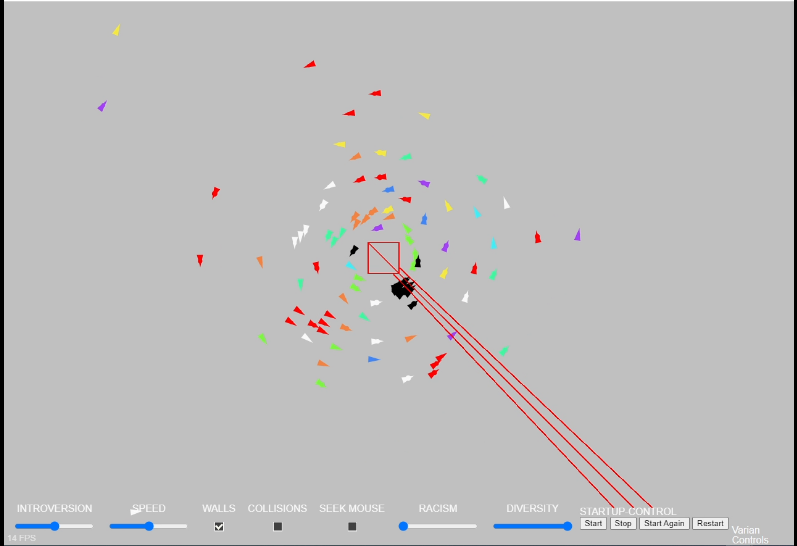
\includegraphics[scale=0.4]{gambar/gambar4tawafflocking25variabel}}

\subfigure[Grafik Model Flocking dengan range 25 N=100 gaya dominan tawaf]{\label{fig:flocking dengan range 25 dominan force}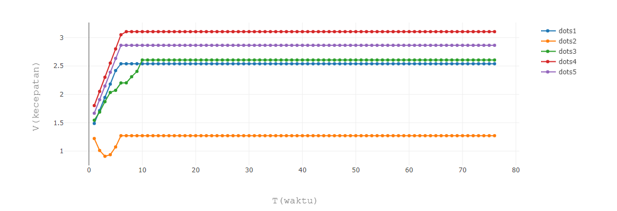
\includegraphics[scale=0.3]{gambar/datagrafik/range25heterogen}}


\subfigure[Model Flocking dengan range 50 N=100 gaya dominan tawaf]{\label{fig:flocking dengan range 50 dominan force}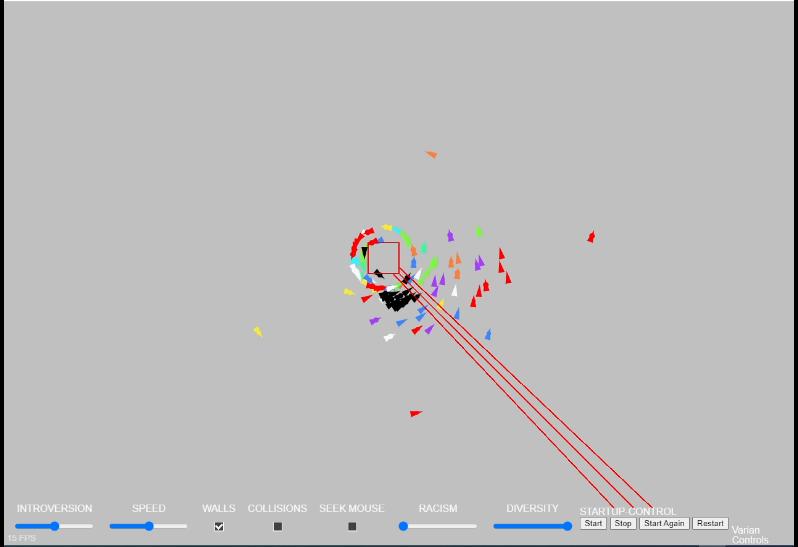
\includegraphics[scale=0.4]{gambar/gambar5tawafflocking50variabel}}

\subfigure[Grafik Model Flocking dengan range 50 N=100 gaya dominan tawaf]{\label{fig:flocking dengan range 50 dominan force}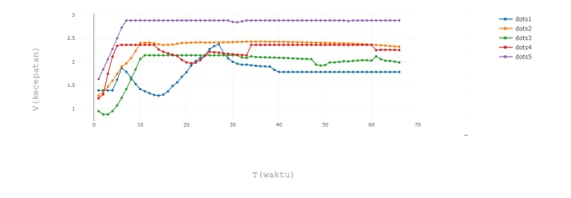
\includegraphics[scale=0.3]{gambar/datagrafik/range50heterogen}}

\caption{Hasil Model alligment,separation dan kohesi dengan range 25 dan range 50 ditambah dengan dominan force tawaf}
\label{fig:2grafikmodel4gaya}
\end{figure}

Dan terakhir pada bagian ini kami menambahkan 2 jenis partikel dengan kecepatan yang berbeda di kedua sistem range yang berbeda. Disini dapat terlihat pada gambar \ref{fig:2grafikmodel4gaya} (kanan) ternyata range yang lebih besar mendistrupsi sistem flocking pada gerakan tawaf. Hal ini dapat terlihat dari partikel yang tertarik menuju pusat. Hasil yang berbeda didapat dari sistem yang menggunakan range lebih kecil \ref{fig:2grafikmodel4gaya}(kiri). Partikel cenderung melakukan menyebar dalam area tawaf dan melakukan flocking dengan lebih optimal. 

Penambahan variabel dari kecepatan partikel ini (merah dengan 1.25 kecepatan partikel biasa) dan (hitam dengan 0.75 partikel biasa). dapat memperlihatkan pada bagian optimal gambar  \ref{fig:2grafikmodel4gaya}(kiri). Bahwa partikel hitam cenderung bergerak di pusat sedangkan partikel merah berada di luar. Hal ini disebabkan karena gaya dominan melebihi gerak flocking.
% \begin{figure}
%      \centering
%      \begin{subfigure}[b]{0.03\textwidth}
%          \centering
%          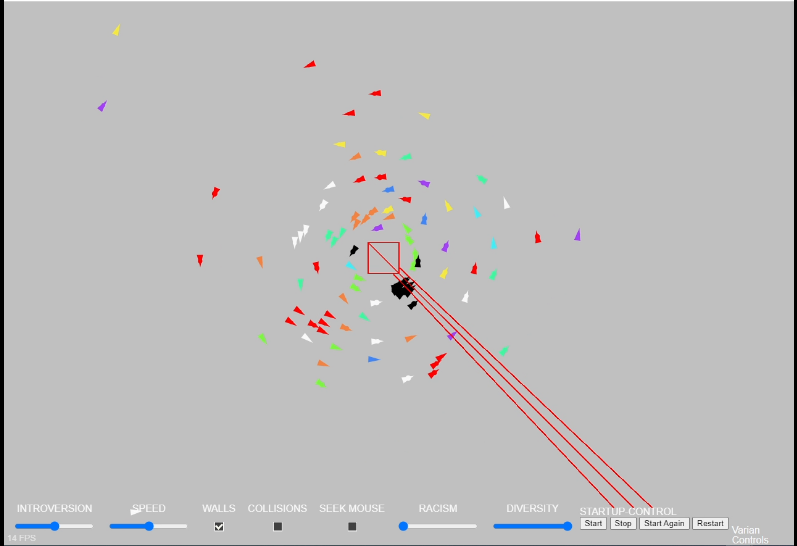
\includegraphics[width=\textwidth]{gambar/gambar4tawafflocking25variabel}
%          \caption{Model Flocking dengan range 25 N=100 Dominan force tawaf}
%          \label{fig:flocking dengan range 25 dominan force}
%      \end{subfigure}
%      \hfill
%      \begin{subfigure}[b]{0.03\textwidth}
%          \centering
%          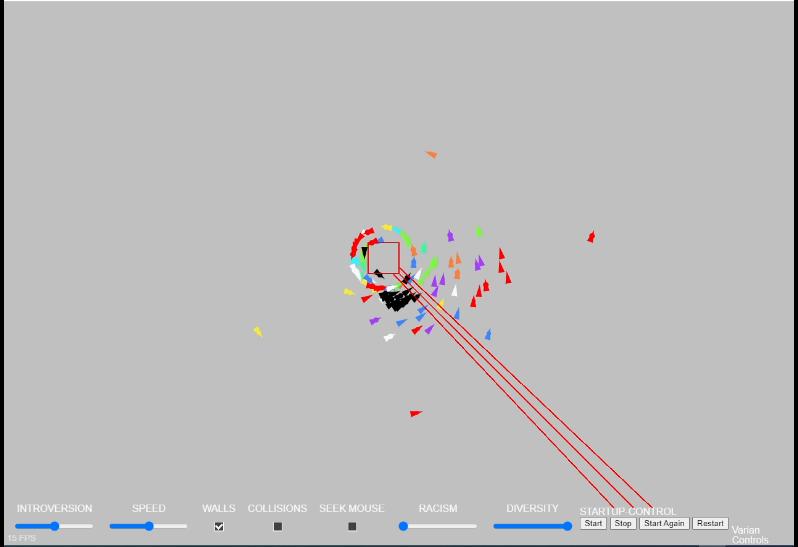
\includegraphics[width=\textwidth]{gambar/gambar5tawafflocking50variabel}
%          \caption{Model Flocking dengan range 50 N=100 Dominan force tawaf}
%          \label{fig:flocking dengan range 50 dominan force}
%      \end{subfigure}
%         \caption{Hasil Model alligment,separation dan kohesi dengan range 25 dan range 50 ditambah dengan dominan force tawaf}
%         \label{fig:2 grafik model 4 gaya}
% \end{figure}
%%%%%%%%%%%%%%%%%%%%%%%%%%%%%%%%%%%%%%%%%%%%%%%%

% \subsection{Optimasi circular  motion dengan partikel Karakteristik}
% \begin{figure}
% \centering
% 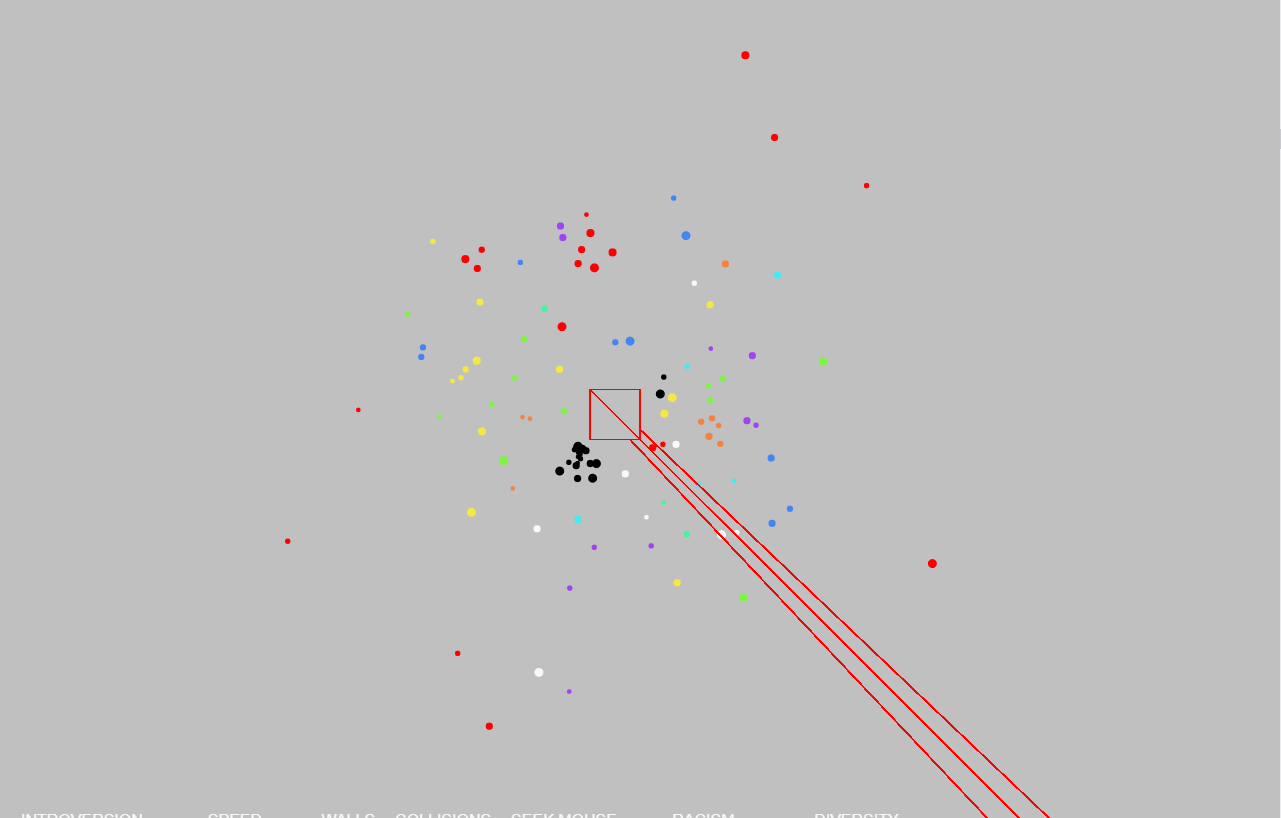
\includegraphics[scale=0.4]{gambar/speed1.5dan0.75.PNG}
% \caption{Hasil Model dengan partikel speed 1.5(merah) dan partikel speed 0.75(hitam)  }
% \end{figure}
% \hspace{0.6cm}Pada Flocking 
%%%%%%%%%%%%%%%%%%%%%%%%%%%%%%%%%%%%%%%%%%%%%%%
\begin{figure}
\centering
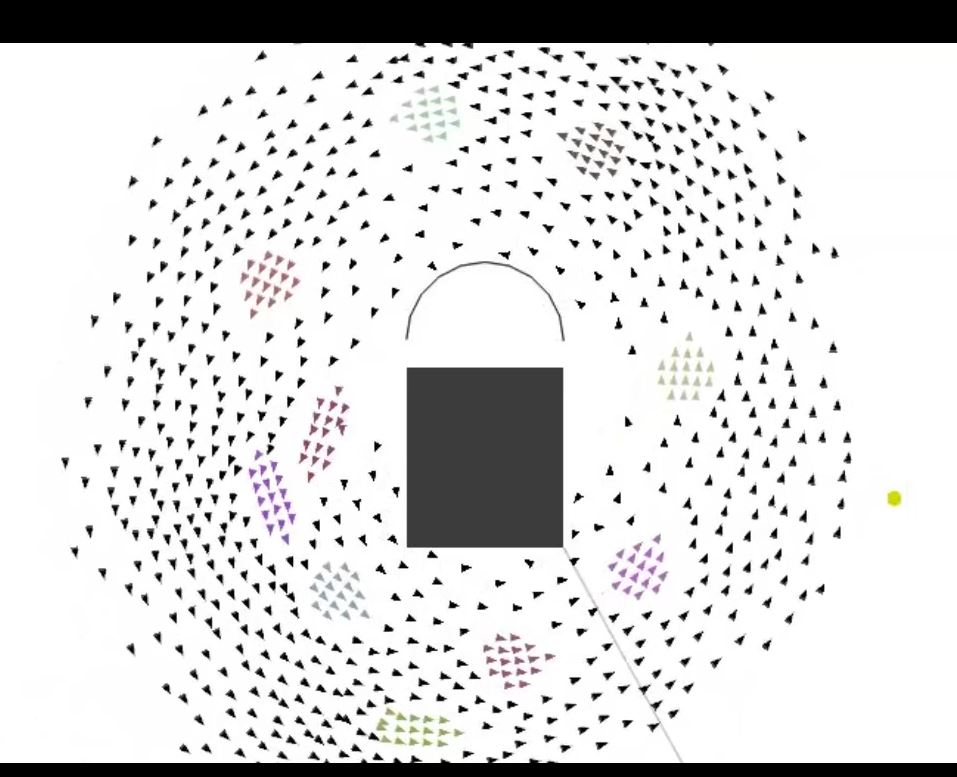
\includegraphics[scale=0.4]{gambar/PaperNasir.JPG}
\caption{Hasil model oleh Nasir}
\label{fig:nasir1}
\end{figure}
\hspace{0.6cm}Bentuk model tawaf dari nasir\citep{Nasir2016} ditunjukan pada gambar diatas. Perilaku partikel berkelompok pada nasir memiliki kecepatan yang sama atau tidak lebih cepat dari partikel sekitarnya. Hal ini yang membuat formasi lebih solid, jika dibandingkan.

\hspace{0.6cm} Hasil penelitian yang telah dilakukan oleh \citep{Nasir2016} ditunjukan oleh \ref{fig:nasir1}. Lingkungan yang dimiliki partikel diletakan kabah berbentuk persegi bersama dengan area bidang perisai untuk hijir ismail. Partikel bergerak berkelompok bersama dengan partikel sejenis dan membuat gerakan tawaf. Hal ini jika dibandingkan dengan dengan hasil pada \ref{fig:2grafikmodel4gaya}(kiri) terdapat banyak perbedaan, diantaranya pergerakan partikel yang cenderung lebih mendekati pusat gaya(kaaba) dan kelompok lebih dapat terpencar, kemudian membuat kelompok yang lebih kecil lagi.

\begin{figure}
\centering
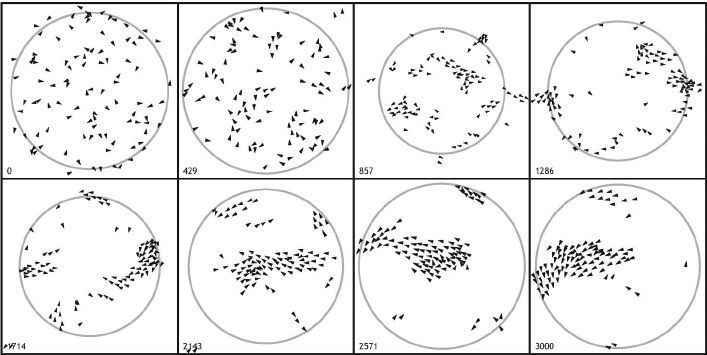
\includegraphics[scale=0.4]{gambar/Bajec.PNG}
\caption{Hasil Flocking Bajec}
\label{fig:bajec1}
\end{figure}
\hspace{0.6cm}Hasil penelitian yang telah dilakukan oleh \citep{Bajec2007} ditunjukan oleh \ref{fig:bajec1}. Area bergerak yang dimiliki partikel berbentuk lingkaran, Ketika partikel melewati batas tersebut maka akan ada gaya yang memaksanya bergerak kembali ke dalam. Jika dibandingkan antara hasil pada Gambar \ref{fig:2grafikmodel3gaya}  dengan Gambar \ref{fig:bajec1}, maka tidak jauh berbeda. Hal ini terlihat dari pola gerak partikel yang pada awalnya tidak berkelompok kemudian menjadi berkelompok dengan beberapa kelompok kecil dan satu kelompok terbesar. 


%\input{referensi}
%\end{document}%bab 4
%\input{format}
%\begin{document}
\chapter{PENUTUP}\label{cha:penutup}
\section{Kesimpulan}

\hspace{0.5cm} Berdasarkan hasil penelitian dan study literatur dapat disimpulkan sementara bahwa:

\begin{enumerate} 
\item  Pergerakan tawaf seperti nasir dengan partikel dapat flocking(mencapai kecepatan yang tetap), dapat membentuk group dan mengelilingi Kaaba, sedangkan skema dalam bergerak mendekati hasil dari kim
\item  Pergerakan partikel berkelompok yang dapat mendekati Kaaba(terutama pada partikel hitam dalam optimasi). 
\item  Penggunakan runge-kutta,dikunakan untuk pemedatan data dalam bentuk grafik. Berdasarkan simulasi yang telah dilakukan.
\end{enumerate} 


\newpage
\section{Saran}\label{cha:saran}
% \begin{enumerate}
% \item partikel lain juga mengikuti Gerakan partikel grouping mendekati pusat Kaaba.
% \item Dalam beberapa case partikel sering melakukan resultan gerak berlawanan arah(mungkin perlu gaya tambahan untuk mendukung arah partikel agar mengelilingi).
% \item Skema ruang partikel mungkin harus diperbesar Bersama dengan Kaaba pusatnya hingga mirip dengan paper nasir

% \end{enumerate}
\hspace{0.5cm} Penelitian ini hanya berfokus pada pembuatan mekanisme flocking pada gerak tawaf. Faktor-faktor fisis seperti gesekan partikel dengan medium yang dilalui dan bentuk skema sebelum tawaf terjadi tidak diperhitungkan. Begitu juga dengan object yang ada dalam garis tawaf sebenarnya kecuali kaaba sebagai pusat gaya. 

%\end{document}%bab 5
\cleardoublepage
\phantomsection
\addcontentsline{toc}{chapter}{DAFTAR PUSTAKA}
\bibliography{file/dafpus} %%daftar pustaka, gunakan ekstensi file .bib, bisa gunakan software mendeley atau download langsung dari link paper 
\chapter*{\indexname}\addcontentsline{toc}{chapter}{\indexname}
\textbf{A}\\
Alignment \textbf{bab} 2;\\
\textbf{B}\\
Boids \textbf{bab} 1 behavioral system \textbf{bab}; bajec \textbf{bab} 4;\\
\textbf{C}\\
Craig Reynolds \textbf{bab} 1; Current State Properties \textbf{bab} 2; Cohesion bab 2; CSS \textbf{bab} 3; Circular Motion \textbf{bab} 2,\textbf{bab} 4\\
\textbf{D}\\
Distribusi Normal \textbf{bab} 2;\\
\textbf{F}\\
Flocking \textbf{bab} 1; fluid dynamic model \textbf{bab} 1;\\
\textbf{G}\\
Gaya Dominan \textbf{bab} 2;\\
\textbf{H}\\
HTML \textbf{bab} 3;\\
\textbf{J}\\
JavaScript \textbf{bab} 3;\\
\textbf{O}\\
Order Parameter \textbf{bab} 2;\\
\textbf{P}\\
victorjs \textbf{bab} 2;\\
\textbf{R}\\
Runge-Kutta \textbf{bab} 2;\\
\textbf{S}\\
SPP \textbf{bab} 2; Separation \textbf{bab} 2; Step Size \textbf{bab} 2;\\
\textbf{T}\\
Tawaf \textbf{bab} 1;\\
\textbf{V}\\
Vicsek \textbf{bab} 1;\\
\textbf{W}\\
Weighting Factor \textbf{bab} 2;\\

% Air \textbf{bab} 1;
% Air Laut \textbf{bab} 1;
% Air Hujan \textbf{bab} 1;
% Air Tanah \textbf{bab} 2;
% Archie \textbf{bab} 2;
% Arus Listrik \textbf{bab} 2;
% Aerasi \textbf{bab} 2;
% aliran \textbf{bab} 2;
% Aluvium \textbf{bab} 4;
% Aquifer \textbf{bab} 4;
% \\\\\textbf{B}\\
% Bumi \textbf{bab} 1;
% Batuan \textbf{bab} 2;
% Beda Potensial \textbf{bab} 2;
% \\\\\textbf{D}\\
% Daratan \textbf{bab} 1;
% Dielektrik \textbf{bab} 2;
% \\\\\textbf{E}\\
% Elektroda \textbf{bab} 2;
% ELektronik \textbf{bab} 2;
% Elektrolitik \textbf{bab} 2;
% \\\\\textbf{F}\\
% Fluida \textbf{bab} 2;
% formusi \textbf{bab} 2;
% \\\\\textbf{G}\\
% Geofisika \textbf{bab} 1;
% Geolistrik \textbf{bab} 2;
% Geometri \textbf{bab} 2;
% GPS \textbf{bab} 3;
% GeoRes \textbf{bab} 3;
% \\\\\textbf{H}\\
% Horizontal \textbf{bab} 2;
% Hujan \textbf{bab} 2;
% Homogen \textbf{bab} 2;
% \\\\\textbf{I}\\
% Interpretasi \textbf{bab} 1;
% Isolator \textbf{bab} 2;
% Ion-ion \textbf{bab} 2;
% Isotropis \textbf{bab} 2;
% Inversi \textbf{bab} 4;
% Iterasi \textbf{bab} 4;
% \\\\\textbf{J}\\
% Jarak \textbf{bab} 2;
% \\\\\textbf{K}\\
% Konduktivitas \textbf{bab} 2;
% Konduktor \textbf{bab} 2;
% Konduksi \textbf{bab} 2; 
% Kedalaman \textbf{bab} 2;
% Konfigurasi \textbf{bab} 2;
% \\\\\textbf{L}\\
% Lokasi \textbf{bab} 1;
% Listrik \textbf{bab} 2;
% Lapisan \textbf{bab} 2;
% Litologi \textbf{bab} 4;
% Lintasan \textbf{bab} 4;
% \\\\\textbf{M}\\
% Mineral  \textbf{bab} 2;
% Material \textbf{bab} 2;
% Molikuler \textbf{bab} 2;
% \\\\\textbf{N}\\
% Notepad \textbf{bab} 3;
% \\\\\textbf{P}\\
% Permukaan \textbf{bab} 1;
% Potensial \textbf{bab} 2;
% Porositas \textbf{bab} 2;
% Pori-Pori \textbf{bab} 2;
% Permeabilitas \textbf{bab} 2;
% Porous \textbf{bab} 2;
% penghantar \textbf{bab} 2;
% Penampang \textbf{bab} 4;
% \\\\\textbf{R}\\
% Resistivitas \textbf{bab} 2;
% Resistivitas Semu \textbf{bab} 2;
% Rembesan \textbf{bab} 2;
% Resitensi \textbf{bab} 2;
% Rongga-rongga \textbf{bab} 2;
% Range \textbf{bab} 2;
% Res IP 2100 \textbf{bab} 3;
% Res2DIV \textbf{bab} 3;
% \\\\\textbf{S}\\
% Saturasi \textbf{bab} 2;
% Semikonduktor \textbf{bab} 2;
% \\\\\textbf{T}\\
% Tahanan \textbf{bab} 2;
% Tegangan \textbf{bab} 2;
% \\\\\textbf{V}\\
% Vertikal \textbf{bab} 2;
% Volt \textbf{bab} 2;
% Volume \textbf{bab} 2;
% \\\\\textbf{W}\\
% Wenner Alpha\textbf{bab} 2;
% Wenner-Sclumberger\textbf{bab} 2;
%LAMPIRAN
\appendix
% \userpackeage{listings}
\titleformat{\chapter}[display] {\normalfont\huge\bfseries\centering} {Lampiran \thechapter}{12pt}{\LARGE}
\clearpage
\renewcommand\bibname{LAMPIRAN}\addcontentsline{toc}{chapter}{LAMPIRAN}
\chapter{sumber kode}
\section{Kode Program gambarBoids.js}
\begin{lstlisting}
function draw(){
	var c = arguments[0];
	var ctx = c.getContext("2d");
	let x=arguments[1];
	let y=arguments[2];
	let vx=arguments[3];
	let vy=arguments[4];
	let radius=arguments[5];
	let sudut1=arguments[6];
	let sudut2=arguments[7];
	let colored =arguments[8];
	let r=5; //3
	let theta=1*Math.atan2(vy,vx) + Math.PI / 2;
	ctx.save();
	ctx.beginPath();
	ctx.translate(x,y);
	ctx.rotate(theta);
	//ctx.fillStyle="rgba(255,000,000,1)"; //this.color
	ctx.fillStyle= colored;
	//ctx.arc(0,0,radius,-sudut1,-sudut2,true);
	//ctx.arc(0,0,radius,1.2*Math.PI,1.8*Math.PI);
	ctx.moveTo(0,-r*2);
	ctx.lineTo(r,r*2);
	ctx.lineTo(-r,r*2);
	ctx.lineTo(0,-r*2);
	ctx.fill();
	ctx.closePath();
	ctx.restore();
	//draw(caOut,X,Y,f[i].vx,f[i].vy,radiusA,sudut1,sudut2);
}
function clear(){
	var ca = arguments[0];
	var ctx = ca.getContext("2d");
	ctx.beginPath();
	ctx.clearRect(0,0,caOut.width,caOut.height);
	ctx.closePath();
}
\end{lstlisting}
\section{Kode Program sides2.js}
\begin{lstlisting}
class Sides2 {
	//create constructor
	constructor() {
		if(arguments.length == 0){
			this.p = [
			new Vect3(),
			new Vect3()
			];
		} else if(arguments.length == 2) {
			this.p = [
			arguments[0],
			arguments[1]
			];
		} else if(arguments.length == 1){
			if(arguments[0] instanceof Sides2)
			this.p = [
				arguments[0].p[0],
				arguments[0].p[1]
			];
		}
	}
	// Get string value
	strval() {
		var s = "(";
		s += this.p[0].strval() + ", ";
		s += this.p[1].strval() + ", ";
		// s += this.p[2].strval() + ", ";
		// s += this.p[3].strval() + ", ";
		s += ")";
		return s;
	}
	
	// Get center coordinate
	center() {
		var N = this.p.length;
		var p0 = new Vect3();
		for(var i in this.p) {
			p0 = Vect3.add(p0, this.p[i]);
		}
		p0 = Vect3.div(p0, N);
		return p0;
	}
}
\end{lstlisting}
\section{vect3.js}
\begin{lstlisting}
/*
	vect3.js
	Vector in 3-d Cartesian coordinate system
	
	Sparisoma Viridi | dudung@gmail.com
	
	20171226
	Create this object (again).
	20171227
	Add some comments for clearer documentation.
*/

// Define class of Vect3
class Vect3 {
	// Create three different types of constructor
	constructor() {
		if(arguments.length == 0) {
			this.x = 0.0;
			this.y = 0.0;
			this.z = 0.0;
		} else if(arguments.length == 3) {
			this.x = arguments[0];
			this.y = arguments[1];
			this.z = arguments[2];
		} else if(arguments.length == 1) {
			if(arguments[0] instanceof Vect3)
			this.x = arguments[0].x;
			this.y = arguments[0].y;
			this.z = arguments[0].z;
		}
	}
	
	// Get string value
	strval() {
		var s = "(";
		s += this.x + ", ";
		s += this.y + ", ";
		s += this.z;
		s += ")";
		return s;
	}
	
	// Add some Vect3
	static add() {
		var N = arguments.length;
		var x = 0.0;
		var y = 0.0;
		var z = 0.0;
		for(var i = 0; i < N; i++) {
			x += arguments[i].x;
			y += arguments[i].y;
			z += arguments[i].z;
		}
		var p = new Vect3(x, y, z);
		return p;
	}
	
	// Substract two Vect3
	static sub() {
		var x = arguments[0].x - arguments[1].x;
		var y = arguments[0].y - arguments[1].y;
		var z = arguments[0].z - arguments[1].z;
		var p = new Vect3(x, y, z);
		return p;
	}
	
	// Multiply Vect3 with scalar or vice versa
	static mul() {
		var a = arguments[0];
		var b = arguments[1];
		var x, y, z;
		if(a instanceof Vect3) {
			x = a.x * b;
			y = a.y * b;
			z = a.z * b;
		} else if(b instanceof Vect3) {
			x = a * b.x;
			y = a * b.y;
			z = a * b.z;
		}
		var p = new Vect3(x, y, z);
		return p;
	}
	
	// Divide Vect3 with scalar
	static div() {
		var a = arguments[0];
		var b = arguments[1];
		var	x = a.x / b;
		var	y = a.y / b;
		var	z = a.z / b;
		var p = new Vect3(x, y, z);
		return p;
	}
	
	// Dot two Vect3
	static dot() {
		var a = arguments[0];
		var b = arguments[1];
		var	xx = a.x * b.x;
		var	yy = a.y * b.y;
		var	zz = a.z * b.z;
		var d = xx + yy + zz;
		return d;
	}
	
	// Cross two Vect3
	static cross() {
		var a = arguments[0];
		var b = arguments[1];
		var	x = a.y * b.z - a.z * b.y;
		var	y = a.z * b.x - a.x * b.z;
		var	z = a.x * b.y - a.y * b.x;
		var p = new Vect3(x, y, z)
		return p;
	}
	
	// Get length of a Vect3
	len() {
		var l = Math.sqrt(Vect3.dot(this, this));
		return l;
	}
	
	// Get unit vector of a Vect3
	unit() {
		var l = this.len();
		var p = Vect3.div(this, l);
		return p;
	}

	// create for 2d cross
	static cross(){
		var a = arguments[1];
		var b = arguments[2];
		var x = (a.x*b.y) - (a.y*b.x);
		var p = new Vect3() 
	}

}

\end{lstlisting}
\section{Kode Program index.html}
\begin{lstlisting}
<!DOCTYPE html>
<html lang="en">
<head>
	<meta charset="utf-8">
	<title>BOIDS!</title>
	<link rel="stylesheet" href="css/style.css">
	<!--[if IE]>
		<script src="http://html5shiv.googlecode.com/svn/trunk/html5.js"></script>
	<![endif]-->
	<script src="https://cdn.plot.ly/plotly-latest.min.js"></script>
</head>

<body id="home">

  <div id="boids-wrapper">
    <canvas id="boids"></canvas>
		<div id="boids-controls-container">
			<div id="mobile-boids-controls">
				<button id="introversion-mobile">Introversion</button>
				<button id="speed-mobile">Speed</button>
				<button id="walls-mobile" class="boids-checkbox-on">Walls</button>
				<button id="collisions-mobile">Collisions</button>
				<button id="mouse-seek-mobile">Seek Mouse</button>
				<button id="racism-mobile">Racism</button>
				<button id="diversity-mobile">Diversity</button>
			</div>
			<div id="introversion-control-container" class="boids-control boids-control-range">
				<span class="boids-control-close"></span>
				<div class="range-slider">
					<label for="introversion"><p>Introversion</p></label>
					<input class="input-range" type="range" step="1" value="5" min="0" max="10" name="introversion" id="introversion">
			    <span class="range-value"></span>
				</div
>			</div>
			<div id="speed-control-container" class="boids-control boids-control-range">
				<span class="boids-control-close"></span>
				<div class="range-slider">
					<label for="introversion"><p>Speed</p></label>
					<input class="input-range" type="range" step="1" value="5" min="0" max="10" name="speed" id="speed">
			    <span class="range-value"></span>
				</div>
			</div>
			<div class="boids-control boids-control-checkbox">
				<div class="checkbox">
					<p>Walls</p>
					<input type="checkbox" id="walls" name="walls"/>
					<label for="walls"></label>
				</div>
			</div>
			<div class="boids-control boids-control-checkbox">
				<div class="checkbox">
					<p>Collisions</p>
					<input type="checkbox" id="collision-detection" name="collision-detection"/>
					<label for="collision-detection"></label>
				</div>
			</div>
			<div class="boids-control boids-control-checkbox">
				<div class="checkbox">
					<p>Seek Mouse</p>
					<input type="checkbox" id="mouse-seek" name="mouse-seek"/>
					<label for="mouse-seek"></label>
				</div>
			</div>
			<div id="racism-control-container" class="boids-control boids-control-range">
				<span class="boids-control-close"></span>
				<div class="range-slider">
					<label for="introversion"><p>Racism</p></label>
					<input class="input-range" type="range" step="1" value="0" min="0" max="10" name="racism" id="racism">
			    <span class="range-value"></span>
				</div>
			</div>
			<div id="diversity-control-container" class="boids-control boids-control-range">
				<span class="boids-control-close"></span>
				<div class="range-slider">
					<label for="introversion"><p>Diversity</p></label>
					<input class="input-range" type="range" step="1" value="8" min="1" max="8" name="diversity" id="diversity">
			    <span class="range-value"></span>
				</div>
			</div>
			<div id="fps">
				<p><span id="fps-number"></span> fps</p>
			</div>

			<div class="startup-control">
				
					<p>Startup-Control</p>
					<button id="Start" onlick="startSimu()">Start</button>
					<button id="Stop" onlick="stopSimu()">Stop </button>
					<button>Start Again</button>
					<button>Restart</button>
				</div>
			</div>
			<div id="varian-">
			<p>Varian Controls</p>
		</div>



	</div>
	<p >Varian Controls</p>
  <script src="js/sides2.js"></script>
  <script src="js/vect3.js"></script>
  <script src="js/victor.min.js"></script>
  <script src="js/script.js"></script>
  <script src="js/boid.js"></script>
  <script src="js/gambarBoids.js"></script>
  
</body>
</html>

\end{lstlisting}
\section{Kode Program boids.js}
\begin{lstlisting}
class Boid {

 //constructor boids
  constructor(boid) {

    // Initial Properties
    this.id = boid.id;

    this.position = new Victor( boid.x, boid.y );
    this.positionI = new Victor();

    // for loop
    this.k1 = new Victor();
    this.k2 = new Victor();
    this.k3 = new Victor();
    this.k4 = new Victor();
    this.bun = new Victor();
    this.h = new Victor(1,1);
    this.half = new Victor(0.5,0.5);
    this.two = new Victor(2,2);
    this.Six = new Victor(6,6);
    //

    this.positionTheta = Math.atan2();
    this.distanceFromCenter0 = this.position.distance(center);
    this.coordinateO = new Victor (0,0);
    this.x ;
    this.y ;

    this.radius = boid.radius * radiusCoefficients[ boid.radiusCoefficient ];
    this.introversionCoefficient = boid.introversionCoefficient;
    this.introversion = boid.introversion * this.introversionCoefficient;
    this.quicknessCoefficient = boid.quicknessCoefficient;
    this.quickness = boid.quickness * this.quicknessCoefficient;
    this.racismCoefficient = boid.racismCoefficient;
    this.racism = boid.racism * boid.racismCoefficient;
    this.color = boid.color;
    this.volume = (4/3) * Math.PI * Math.pow( this.radius,3 );

;
    this.angle;
    this.angle2 = 3/2*Math.PI;    


    this.distanceFromCenter = this.position.clone().distance(center);
    this.distanceFromCenter = this.position.distance(center);

    this.positionC = new Victor( this.distanceFromCenter*Math.cos(this.angularVelocity),this.distanceFromCenter*Math.sin(this.angularVelocity));
    this.theta = 0; 
    this.frequency = 0 ;
    this.radians =  Math.PI*2;//*Math.random();

    // Speed & Velocity & Force
    this.maxSpeed = speedIndex * this.quickness;
    this.speed = this.maxSpeed * .5;
    this.speedangular = this.speed/this.distanceFromCenter;

    this.angularVelocity = this.speed/this.distanceFromCenter;
 
    var radians = Math.PI; //* getRandomInt(-99,100) / 100;
 
    this.velocity = new Victor( this.speed * Math.cos( radians ), this.speed * Math.sin( radians ) )
    this.velocity0 = new Victor(Math.cos(this.radians)*this.distanceFromCenter,Math.sin(this.radians)*this.distanceFromCenter);
  //Force and Accel
    this.maxForce = 0.25//.5;
    this.maxForce2 = .1;
    this.acceleration = new Victor(0,0);
    this.angularAcceleration;
    this.desiredPosition;
    this.target;
  }
////////////// meta transform
    transform() {
    var realPosition = transform({x:this.position.x ,y:this.position.y});

  }
////////////////

  seek( target ){
    var targetposition = target.clone();
    var diff = targetposition.subtract(this.position);
    var desired = new Victor(diff.x,diff.y);
    this.desiredPosition = desired;
    this.target = diff;

    //area buffer seek biar seaknya beda
    if (target.radius) {
      var buffer = target.radius + this.radius + 1;
    } else {
      var buffer = this.radius * 2 + 1;
    }
    //
    var dist = diff.magnitude();
    if (dist < buffer) {
      desired.x = 0;
      desired.y = 0;
    } else if ( dist <= 100 ) {
      //normalize and multiply
      desired.normalize();
      desired.divide({x:this.maxSpeed * dist / 100,y:this.maxSpeed * dist / 100});
    } else {
      desired.limitMagnitude(this.maxSpeed);
    }
    desired.subtract(this.velocity);
    desired.limitMagnitude(this.maxForce);
    return desired;
  }

  //this must edited to seek center canvas target position
   centripetal( boids ){
    var sum = new Victor();
    var steer = new Victor();
    var u = new Victor(100,100);
    var t = 0,dt=1;
    for (var i = 0; i < boids.length; i++) {
      var desiredtoCenter = Math.pow(this.velocity,2)/distanceFromCenter;
      var nowPosition = this.position.clone();
      var vecKaaba = Victor.fromObject(wallsKaaba);
      var distanceFromCenter =this.position.clone().distance(center); //hajar aswad

      var centerKaaba = new Victor(surf.center().x,surf.center().y);
      var distanceFromCenter2 = this.position.clone().distance(centerKaaba);
      var pathCircular = 2*Math.PI* distanceFromCenter;
      var theta = 1;

   
        var N = sides.length;
        
        if ( (distanceFromCenter2 > 0 &&distanceFromCenter2 < 50) ) {//distanceFromCenter2 > 0 &&distanceFromCenter2 < 50

      
        var thisposition = this.position.clone();
        var diff = thisposition.subtract(centerKaaba);
        var diffVelocity = diff;
        diff.normalize();
        diff.multiply({x:distanceFromCenter,y:distanceFromCenter});
    
        sum.add(diff);
        t+=dt
        }
        //force to area that make boids circular path 
        if ( (distanceFromCenter2 > 50 && distanceFromCenter2 <= 500 ) ) {

        var thisposition = this.position.clone();
        var diff = thisposition.subtract(centerKaaba);
 
        const diffVelocity = diff;

        diff.normalize();
        diff.multiply({x:distanceFromCenter,y:distanceFromCenter});

        sum.subtract(diff);

        t+=dt
        }else{

        }
        // 
      //}
      
    }
    if (t > 0) {
      sum.divide({x:t,y:t});
      sum.normalize();
      sum.multiply({x:this.maxSpeed,y:this.maxSpeed});
      steer = sum.add(this.velocity);
      steer.limitMagnitude(this.maxForce);
      return steer;
    } else {
      return steer;
    }
  }


    circularMotion( boids ){
    var sum = new Victor();
    var steer = new Victor();
    var t = 0,dt=1;
    for (var i = 0; i < boids.length; i++) {

      var desiredtoCenter = Math.pow(this.velocity,2)/distanceFromCenter;
      var distanceFromCenter =this.position.clone().distance(center);

      var pathCircular = 2*Math.PI* distanceFromCenter;
      var theta = 1;
      
      if ( (distanceFromCenter < 50 && distanceFromCenter < 300 ) ) {
        var thisposition = this.position.clone();
        var thisvelocity = this.velocity.clone();
        var thispositionX = thisposition.x + (distanceFromCenter*Math.sin(toRadian(1)));
        var thispositionY = thisposition.y + (distanceFromCenter*Math.cos(toRadian(1)));
        var diff = thisposition.add(new Victor(thispositionX,thispositionY));
        diff.normalize();

        sum.add(diff);
        t+=dt
      }
    }
    if (t > 0) {
      sum.divide({x:t,y:t});
      sum.normalize()
      sum.multiply({x:this.maxSpeed,y:this.maxSpeed});
      steer = sum.subtract(this.velocity);
      steer.limitMagnitude(this.maxForce);
      return steer;
    } else {
      return steer;
    }
  }


  separate( boids ){
    var sum = new Victor();
    var t = 0,dt=1;
    
    for (var j = 0; j < boids.length; j++) {
      if ( this.color != boids[j].color ) {
        var racismMultiplier = this.racism;
      } else {
        var racismMultiplier = 0;
      }
      var desiredSeparation = this.radius + boids[j].radius + ( 25 * this.introversion ) + ( 50 * racismMultiplier );
      var sep = this.position.clone().distance(boids[j].position);
      if ( (sep > 0) && (sep < desiredSeparation) ) {
        var thisposition = this.position.clone();
        var diff = thisposition.subtract(boids[j].position);
        diff.normalize();
        diff.divide({x:sep,y:sep});
        sum.add(diff);
        t+=dt
      }
    }
    if (t > 0) {
      sum.divide({x:t,y:t});
      sum.normalize();
      sum.multiply({x:this.maxSpeed,y:this.maxSpeed});
      sum.subtract(this.velocity);
      sum.limitMagnitude(this.maxForce);
    }
    return sum;
  }

 
  align( boids ) {
    var neighborDist = 50;//50
    var sum = new Victor();
    var steer = new Victor();
    var t = 0,dt=1;
    for (var i = 0; i < boids.length; i++) {
      var dist = this.position.distance(boids[i].position);
      if ( dist > 0 && dist < neighborDist ) {
        sum.add(boids[i].velocity);
        t+=dt;
      }
    }
    if (t > 0) {
      sum.divide({x:t,y:t});
      sum.normalize()
      sum.multiply({x:this.maxSpeed,y:this.maxSpeed});
      steer = sum.subtract(this.velocity);
      steer.limitMagnitude(this.maxForce);
      return steer;
    } else {
      return steer;
    }
  }


  cohesion( boids ) {
    var neighborDist = 50;//50
    var sum = new Victor();
    var t = 0,dt=1;
    for (var i = 0; i < boids.length; i++) {
      var dist = this.position.distance(boids[i].position);
      if ( dist > 0 && dist < neighborDist ) {
        sum.add(boids[i].position);
        t+=dt;
      }
    }
    if (t > 0) {
      sum.divide({x:t,y:t});
      return this.seek(sum);
    } else {
      return sum;
    }
  }


  avoidWalls() {

    var buffer = mobile ? 5 : 15;

    if ( this.distanceFromHorWall() < this.radius * buffer || this.distanceFromVertWall() < this.radius * buffer ) {
      return this.seek(center);
    } else { return false; }

  }


  flock() {

    // Get Forces

    var alignForce = this.align(boids);
    //console.log(alignForce);

    var circularMotionForce = this.circularMotion(boids);
    if ( mouseSeek ){ 
      var mouseForce = this.seek(center);//mouse.position
      var x = new Victor(0,0 );
      var mouseForce2 = this.seek(x);
    }
    //if ( mouseSeek ) var mouseForce = this.seek(mouse.position);//mouse.position
    var separateForce = this.separate(boids);
    var cohesionForce = this.cohesion(boids);
    ///
    var centripetalForce = this.centripetal(boids);
    ////
    if ( walls ) var avoidWallsForce = this.avoidWalls();


    // Weight Forces
    var centripetalWeight = 1;
    var circularWeight = 1;
    //
    var alignWeight = 1; //1.2
    if ( mouseSeek ) var mouseWeight = 0.5; //.2
    var separateWeight = 1;
    var cohesionWeight = 1;
    if ( walls ) var avoidWallsWeight = 1.2;

    // Apply forces
    
    this.applyForce( alignForce, alignWeight );
    if ( mouseSeek ){ 
      this.applyForce( mouseForce, mouseWeight );
      this.applyForce( mouseForce2, mouseWeight );
    }
    this.applyForce( separateForce, separateWeight );
    this.applyForce( cohesionForce, cohesionWeight );
    //
    //this.applyForce(centrifugalForce, centrifugalWeight );
    this.applyForce(centripetalForce, centripetalWeight );

    //this.applyForce(circularMotionForce, circularWeight );
    //
    var distanceFromCenter =this.position.clone().distance(center);
    
    //
    if ( walls && avoidWallsForce ) this.applyForce( avoidWallsForce, avoidWallsWeight );

  }



  //acceleration
  applyForce( force, coefficient ) {
    if ( ! coefficient ) { var coefficient = 1; }
    force.divide({x:coefficient,y:coefficient});
    this.velocity.add(force);
    this.velocity.limitMagnitude( this.maxSpeed );
  }


    //calculate
  nextPosition() {

    // Update position
    let k1,k2,k3,k4,bun;
    var positiont= this.position.clone(); 
    var velocityt = this.velocity.clone();
    var positiont2= this.position.clone(); 
    var velocityt2 = this.velocity.clone();

    function u(p,v){
      var uv = p.add(v);
      return uv
    }

    const two = new Victor(2,2);
    const h = new Victor(0.5,0.5);
    const p0 = this.position

    var vecP = this.position.toArray();
    var vecV = this.velocity.toArray();
    var fLen=1,jLen=1;
    var upS =[,];
    for (let i = 0; i < vecP.length; i++) {
      for (let j = 0; j < vecV.length; j++){
        upS[i]= vecP[i]+vecV[i];
      }
    }
    




    this.velocity = this.velocity.add(this.acceleration);
    this.positionI = this.position.add(this.velocity);//.multiply(this.h);
    //console.log(this.positionI);
    //////////////////////////////////////////////////////////////////////////////////////////////////////////////////////
    function rk4(x,v){
      var x1 = x;
      var v1 = v;
      //var h1 = h;
      
      var two = new Victor(2,2);
      var h = new Victor(0.5,0.5);
      var Six = new Victor(6,6);

      function f(x0,v0){
        x0.add(v0);
      }
      console.log("TEST"+f(x1.clone(),v1.clone()));
      var k1 = f(x1.clone(),v1.clone()).multiply(h);
      //console.log("k1:"+k1);

      var k2 = f(x1.clone().add(k1.clone().divide(two)),v1.clone().add(h.clone().divide(two))).multiply(h);
      var k3 = f(x1.clone().add(k2.clone().divide(two)),v1.clone().add(h.clone().divide(two))).multiply(h);
      var k4 = f(x1.clone().add(k3),v1.clone.add(h)).multiply(h);
      
      var bun = k1.clone().add(k2.clone().multiply(two)).add(k3.clone().multiply(two)).add(k4).multiply(h).divide(Six);
      //var bun = k1.clone().add(k2.clone().multiply(two)).add(k3.clone().multiply(two)).add(k4).multiply(h);
      //var vN = x1.clone().add(bun.clone().multiply(h).divide(Six));
      var vN = bun
      console.log("V"+vN);
      return(vN);
    }

    //rk4(this.position,this.velocity);
    //console.log("apakah ini:"+rk4(this.position,this.velocity));
    // this.velocity.add(this.h)
    // this.positionI = this.positionI.add(rk4(this.position,this.velocity));
    // console.log("POS"+this.positionI);
    ///////////////////////////////////////////////////////////////////////////////////////////////////////////////////////
    // k1 = (this.position.add(this.velocity)).multiply(this.h);
    // this.k1.copy(k1);
    // console.log("k1"+this.k1);
    // // k2 = positiont.add(k1.divide(this.two)).add(velocityt2).add(this.h.divide(this.two)).multiply(this.h);
    // console.log("k2"+k2);
    // k3 = positiont.add(k2.divide(this.two)).add(velocityt).add(this.h.divide(this.two)).multiply(this.h);
    // k4 = positiont.add(k3).add(velocityt).add(this.h).multiply(this.h);
    // this.bun = k1.add(k2.multiply(this.two)).add(k3.multiply(this.two)).add(k4).divide(this.Six);
    // this.positionI = this.position.add(this.bun);
    // //console.log(this.positionI)
    // console.log(this.position);
    // console.log(this.velocity);
    // this.k1 = this.position.add(this.velocity).multiply(this.h);
    // this.k2 = this.position.add(this.k1.divide(this.two)).add(this.velocity).add(this.h.divide(this.two)).multiply(this.h);
    // this.k3 = this.position.add(this.k2.divide(this.two)).add(this.velocity).add(this.h.divide(this.two)).multiply(this.h);
    // this.k4 = this.position.add(this.k3).add(this.velocity).add(this.h).multiply(this.h);
    //console.log(this.position);

    ////////////////////////////////////////////////
    // this.k1 = this.k1.add(u(this.position,this.velocity)).multiply(h);
    // console.log("k1"+this.k1);
    // this.k2 = this.k2.add(u(this.position.add(this.k1.clone().divide(two)),this.velocity.add(h.divide(two)))).multiply(h);
    // console.log("k2"+this.k2);
    // // this.k3 = this.k3.add(u(this.position.add(this.k2.divide(this.two)),this.velocity.add(this.h.divide(this.two)))).multiply(this.h);
    // console.log("k3"+this.k3);
    // this.k4 = this.k4.add(u(this.position.add(this.k3.clone()),this.velocity.add(this.h))).multiply(this.h);
    // console.log("k4"+this.k4);
    // this.bun = this.k1.clone().add(this.k2.clone().multiply(this.two)).add(this.k3.clone().multiply(this.two)).add(this.k4.clone()).divide(this.Six);
    // console.log("bundle="+this.bun)
    // this.positionI = this.position.add(this.bun);
    ///////////////////////////////////////////////////
    // ///////////////////////////////////////////////////
    // this.k1 = u(this.position.clone(),this.velocity.clone()).multiply(this.h);
    // console.log("k1"+this.k1);
    // this.k2 = u(this.position.clone().add(this.k1.clone().divide(this.two)),this.velocity.clone().add(this.h.clone().divide(this.two))).multiply(this.h);
    // this.k3 = u(this.position.clone().add(this.k2.clone().divide(this.two)),this.velocity.clone().add(this.h.clone().divide(this.two))).multiply(this.h);
    // this.k4 = u(this.position.clone().add(this.k3.clone()),this.velocity.clone().add(this.h)).multiply(this.h);

    // this.bun = this.k1.clone().add(this.k2.clone().divide(two)).add(this.k3.clone().divide(two)).add(this.k4.clone()).divide(this.Six);
    // console.log("test"+bun);
    // this.positionI = this.position.add(this.bun);
    // ////////////////////////////////////////////////////////
    // console.log("p"+this.positionI);
    // // this.velocity.add(this.h);
    // console.log(this.positionI);
    //console.log(this.k1);
    // // this.positionI = this.position.add()
    // var test = new Victor();
    // var u = new Victor(1,3);

    // test = test.add(u).add(u).multiply(h);
    // console.log(test);

    //this.positionI = this.position + 1/6*(k1+(2*k2)+(2*k3)+k4);
    //this.position.y = this.position.y.add(this.velocity.y);
    // k1 = this.position.add(this.velocity).multiply(0.1);
    // k2 = this.position.add(this.velocity.add(0.1/2)).multiply(k1/2).multiply(0.1);
    // k3 = this.position.add(this.velocity.add(0.1/2)).multiply(k2/2).multiply(0.1);
    // k4 = this.position.add(this.velocity.add(0.1)).multiply(k3/2).multiply(0.1);
    // this.position = this.position + 1/6*(k1+(2*k2)+(2*k3)+k4);
   
    // function rungeKutta(){
    // }
    // Loop through behaviors to apply forces

    this.flock();


    // Collision detection if enabled
    //console.log(this.position)
    if ( collisions ) { this.detectCollision(); }

    // Check edges for walls or overruns
    this.edgeCheck();
    //this.kaabaCheck()

  }


  edgeCheck() {
    if (walls) {
      this.wallBounce();
      //this.kaabaBounce();
    } else {
      this.borderWrap();
    }
  }


  borderWrap() {
    if (this.position.x < 0) {
      this.position.x = document.body.clientWidth;
    } else if ( this.position.x > document.body.clientWidth ) {
      this.position.x = 0;
    }
    if (this.position.y < 0) {
      this.position.y = document.body.clientHeight;
    } else if ( this.position.y > document.body.clientHeight ) {
      this.position.y = 0;
    }
  }




  wallBounce() {
    
    if (this.position.x <= this.radius) {
      this.position.x = this.radius;
    } else if ( this.position.x >= document.body.clientWidth - this.radius) {
      this.position.x = document.body.clientWidth - this.radius;
    }
    if (this.position.y <= this.radius) {
      this.position.y = this.radius;
    } else if ( this.position.y >= document.body.clientHeight - this.radius ) {
      this.position.y = document.body.clientHeight - this.radius;
    }
    if ( this.distanceFromHorWall() <= this.radius  ) {
      this.velocity.invertY();
    }
    if ( this.distanceFromVertWall() <= this.radius  ) {
      this.velocity.invertX();
    }
 
  }

 
  distanceFromVertWall() {
    if (this.velocity.x > 0) {
      return document.body.clientWidth - ( this.position.x );
    } else {
      return this.position.x;
    }

  }


  distanceFromHorWall() {
    if (this.velocity.y > 0) {
      return document.body.clientHeight - ( this.position.y );
    } else {
      return this.position.y;
    }
  }

  ///tambahan ikhsan 
  distanceFromHorKaaba(){
    if (this.velocity.y > 0){
      return wallskaaba.y - (this.position.y);
    } else {
      return this.position.y
    }
  }
  distanceFromVertKaaba(){
    if (this.velocity.x > 0) {
      return wallsKaaba.x - (this.position.x);
    } else {
      return this.position.x;
    }
  }

  wallKaabaBounce(){
    if (this.position.x <= this.radius) {
      this.position.x = this.radius;
    } else if ( this.position.x >= document.body.clientWidth - this.radius) {
      this.position.x = document.body.clientWidth - this.radius;
    }
    if (this.position.y <= this.radius) {
      this.position.y = this.radius;
    } else if ( this.position.y >= document.body.clientHeight - this.radius ) {
      this.position.y = document.body.clientHeight - this.radius;
    }
    if ( this.distanceFromHorWall() <= this.radius  ) {
      this.velocity.invertY();
    }
    if ( this.distanceFromVertWall() <= this.radius  ) {
      this.velocity.invertX();
    }

 
  }








  draw(){
    //c.beginPath();
    //transform the position 
    var rr = transform({x:this.positionI.x, y:this.positionI.y}); // tambahan ikhsan transformasi
    var theta = -1*Math.atan2(this.velocity.y,this.velocity.x); + Math.PI /2;
    var vr = transform({x:this.velocity.x, y:this.velocity.y}); // tambahan ikhsan transformasi
    var t,deltat;

    let r = this.radius;
    let sudut1=Math.PI*(0);
    let sudut2=Math.PI*((2/3)-(1/3));
    //let theta =-1*Math.atan2(this.velocity.x,this.velocity.y) + Math.PI /2;
    c.save();
    c.beginPath();


    c.arc(rr.x, rr.y, this.radius, 0, Math.PI * 2);
    c.fillStyle = this.color;
    c.fill();
    c.closePath();
    c.restore();

 
    draw(canvas,rr.x,rr.y,vr.x,vr.y,1,sudut1,sudut2,this.color);
    t=+deltat

 
  }

  startLine(){
    c.strokeStyle = "#ff0000";
    c.beginPath();
    c.moveTo(center.x-50,center.y-50);
    c.lineTo(center.x,center.y);
    c.moveTo(center.x,center.y);
    c.lineTo(1020,820);
    c.moveTo(center.x-10,center.y);
    c.lineTo(988,820);
    c.moveTo(center.x,center.y-10);
    c.lineTo(1050,820);
    //c.fillStyle = "#ff0000";
    c.fill();
    c.stroke();
  }

  drawArrow(){
    c.strokeStyle = "#ff0000";
    c.beginPath();
    c.moveTo(this.position.x,this.position.y);
    c.lineTo(center.x,center.y);
    c.stroke();
  }
  
  update() { 
    //this.transform();// tambahan ikhsan
    var sudut1=Math.PI*(0);
    var sudut2=Math.PI*((2/3)-(1/3));

    this.draw();
    ///draw all boundary except kaaba
    //this.startLine();
    
    //this.circularPath();
    ///
    this.nextPosition();
    c.beginPath();

    c.closePath();

    //this.draw(); //awalnya disini
  }




  detectCollision(){

    for (var i = 0; i < boids.length; i++) {
      if ( this === boids[i] ) { continue; }
      if ( getDistance( this.position.x, this.position.y, boids[i].position.x, boids[i].position.y) - ( this.radius + boids[i].radius ) < 0 ) {
        this.resolveCollision( this, boids[i]);
      }
    }
  }


  rotate(velocity, angle) {
    return {
        x: velocity.x * Math.cos(angle) - velocity.y * Math.sin(angle),
        y: velocity.x * Math.sin(angle) + velocity.y * Math.cos(angle)
    };
  }


   resolveCollision(boid, otherBoid) {

      var xVelocityDiff = boid.velocity.x - otherBoid.velocity.x;
      var yVelocityDiff = boid.velocity.y - otherBoid.velocity.y;

      var xDist = otherBoid.position.x - boid.position.x;
      var yDist = otherBoid.position.y - boid.position.y;

      // Prevent accidental overlap of boids
      if ( xVelocityDiff * xDist + yVelocityDiff * yDist >= 0 ) {

        // Grab angle between the two colliding boids
        var angle = -Math.atan2(otherBoid.position.y - boid.position.y, otherBoid.position.x - boid.position.x);

        // Store mass in var for better readability in collision equation
        var m1 = boid.mass;
        var m2 = otherBoid.mass;

        // Velocity before equation
        var u1 = this.rotate(boid.velocity, angle);
        var u2 = this.rotate(otherBoid.velocity, angle);

        // Velocity after 1d collision equation
        var v1 = { x: u1.x * (m1 - m2) / (m1 + m2) + u2.x * 2 * m2 / (m1 + m2), y: u1.y };
        var v2 = { x: u2.x * (m1 - m2) / (m1 + m2) + u1.x * 2 * m2 / (m1 + m2), y: u2.y };

        // Final velocity after rotating axis back to original position
        var vFinal1 = this.rotate(v1, -angle);
        var vFinal2 = this.rotate(v2, -angle);

        // Swap boid velocities for realistic bounce effect
        boid.velocity.x = vFinal1.x;
        boid.velocity.y = vFinal1.y;
        boid.velocity.limitMagnitude(boid.maxSpeed);

        otherBoid.velocity.x = vFinal2.x;
        otherBoid.velocity.y = vFinal2.y;
        otherBoid.velocity.limitMagnitude(otherBoid.maxSpeed);
      }

    }

}
\end{lstlisting}

\section{Kode Program script.js}
\begin{lstlisting}

/*---- Global Setup ----*/

// Set up canvas
const canvas = document.getElementById('boids');
const c = canvas.getContext('2d');

//Get Firefox
var browser=navigator.userAgent.toLowerCase();
if(browser.indexOf('firefox') > -1) {
  var firefox = true;
}

// Detect Mobile
var mobile = ( /Android|webOS|iPhone|iPad|iPod|BlackBerry|IEMobile|Opera Mini/i.test(navigator.userAgent) ) ? true : false;

// Set Size
var size = {
  width: window.innerWidth || document.body.clientWidth,
  height: window.innerHeight || document.body.clientHeight
}
console.log("ini bodi client"+document.body.clientWidth+"dan"+document.body.clientHeight);
canvas.width = size.width;
canvas.height = size.height;
console.log("besar canvas");
console.log(size.width);
console.log(size.height);

var center = new Victor( size.width / 2 ,size.height / 2 );
console.log("pusat"+center.x);


// Initialize Mouse
var mouse = {
  position: new Victor( innerWidth / 2, innerHeight / 2 )
};

/*---- end Global Setup ----*/

/*---- Helper Functions ----*/

/**
 * Returns a random int between a min and a max
 *
 * @param  int | min | A minimum number
 * @param  int | max | A maximum number
 * @return int | The random number in the given range
 */
function getRandomInt(min, max) {
  return Math.floor(Math.random() * (max - min + 1)) + min;
}

/**
 * Returns the distance between two coordinates
 *
 * @param  int | x1 | Point 1's x coordinate
 * @param  int | y1 | Point 1's y coordinate
 * @param  int | x2 | Point 2's x coordinate
 * @param  int | y2 | Point 2's y coordinate
 * @return int | The distance between points 1 and 2
 */
function getDistance(x1, y1, x2, y2) {
  var xDist = x2 - x1;
  var yDist = y2 - y1;
  return Math.sqrt( Math.pow(xDist, 2) + Math.pow(yDist, 2) );
}

/**
 * Returns a random color from the colors array
 *
 * @param  array | colors | An array of color values
 * @return string | The random color value
 */
function randomColor(colors) {
  return colors[ Math.floor( Math.random() * colors.length) ];
}

/**
 * Get coefficients based on normal distribution
 *
 * @param  int | mean | The mean value of the data set
 * @param  int | stdev | The standard deviation for the data set
 * @return int | A number from the data set
 */
function gaussian(mean, stdev) {
    var y2;
    var use_last = false;
    return function() {
        var y1;
        if(use_last) {
           y1 = y2;
           use_last = false;
        }
        else {
            var x1, x2, w;
            do {
                 x1 = 2.0 * Math.random() - 1.0;
                 x2 = 2.0 * Math.random() - 1.0;
                 w  = x1 * x1 + x2 * x2;
            } while( w >= 1.0);
            w = Math.sqrt((-2.0 * Math.log(w))/w);
            y1 = x1 * w;
            y2 = x2 * w;
            use_last = true;
       }

       var retval = mean + stdev * y1;
       if(retval > 0)
           return retval;
       return -retval;
       console.log("tes retval"+retval);
   }
}

var getCoefficient = gaussian(50, 9); //(50,9)
var getQuicknessCoefficient = gaussian(75,7.5); //(75,7.5)

/**
 * Add Limit Magnitude function to Victor objects
 *
 * @param  int | max | The limit magnitude for the vector
 */
Victor.prototype.limitMagnitude = function (max) {

  if (this.length() > max) {
    this.normalize();
    this.multiply({x:max,y:max});
  }

};
/**
 * Convert angle to radian
 *
 * @param  int | sudut | angle that convert
 */

function toRadian (sudut) {
  return sudut * (Math.PI / 180);
}

/*--- end Helper Functions ----*/

/*---- Loop and Initializing ----*/

// Checkbox Options
var walls = true;
var mouseSeek = false;
var collisions = false;

/*---- How much Boids ----*///120
var allBoids = 100;//1000;
var numAllBoids = allBoids;

var minBoids = 60;//1000;
var numBoids = minBoids;

var agroBoids = 20;//1000;//20
var numAgBoids = agroBoids;

var blackBoids = 20;//20
var numBlBoids =blackBoids;

// Set possible radii  based on screen size
var radius;
if ( size.width / 288 > 5 ) {
  radius = 5;
} else if ( size.width / 288 < 3) {
  radius = 3;
} else {
  radius = size.width / 288;
}
var radiusCoefficients = [.5,.6,.7,.8,.9,1];

// Boid Attributes
var colors = [
  '#4286f4',
  '#7df442',
  '#41f4a0',
  '#f9f9f9',
  '#a341f4',
  '#f48341',
  '#f4e841',
  '#42ebf4'
];

var colorsBlack = [
  '#000000'
];

var colorsRed = [
  '#FF0000'
];

var colorsYellow = [
  ' #FFFF00'
];

var diversity = 8;

var quickness = 1;
var agroQuickness = 1.25;
var blackQuickness = 0.5;

var introversion = .5;
var racism = 1; // 0 awalnya coba 5
var speedIndex;
if ( size.width / 160 < 5 ) {
  speedIndex = 1.25;//5 DEFAULT x
} else if ( size.width / 180 > 8 ) {
  speedIndex = 2.25;//9
} else {
  speedIndex = size.width / 180;
}
var maxForceAggro = 0.4;

// Create Boids Array
var boids = [];

// Other 
var trigger = true;
/**
 * Create Boids Array
 *
 */
function createBoids() {

  // Instantiate all Boids
  for ( i = 0; i < numBoids; i++ ) {

    // Generate introversion coefficient
    var introversionCoefficient = getCoefficient() / 100;
    var quicknessCoefficient = getQuicknessCoefficient() / 100;
    var racismCoefficient = getCoefficient() / 100;
    var radiusCoefficient = Math.floor(Math.random() * radiusCoefficients.length);

    // Generate random coords MUST FROM 50 TO SIZE CANVAS OR WALL MASJIDIL
    // if ( distanceFromCenter > 300 && distanceFromCenter < 1500){
    //   var x = Math.ceil(Math.random()* ( getRandomInt(center.x+50,size.width) - ( radius * 2 ) ) ) + ( radius );//size.width
    //   var y = Math.ceil(Math.random()* ( getRandomInt(center.y+50,size.height) - ( radius * 2 ) ) ) + ( radius );//size.height
    // }
    var x = Math.ceil(Math.random()* ( getRandomInt(center.x+50,size.width) - ( radius * 2 ) ) ) + ( radius );//size.width
    var y = Math.ceil(Math.random()* ( getRandomInt(center.y+50,size.height) - ( radius * 2 ) ) ) + ( radius );//size.height
    // For subsequent boids, check for collisions and generate new coords if exist
    if ( i !== 0 ) {
      for (var j = 0; j < boids.length; j++ ) {
        if ( getDistance(x, y, boids[j].x, boids[j].y) - ( radius + boids[j].radius ) < 0 ) {
          x = Math.ceil(Math.random()* ( getRandomInt(center.x+50,size.width) - ( radius * 2 ) ) ) + ( radius );//size.width
          y = Math.ceil(Math.random()* ( getRandomInt(center.y+50,size.height) - ( radius * 2 ) ) ) + ( radius );//size.height
          j = -1;
        }
      }
    }

    // Add new Boid to array
    boids.push( new Boid( {
      id: i,
      x: x,
      y: y,
      speedIndex: speedIndex,
      radius: radius,
      radiusCoefficient: radiusCoefficient,
      quickness: quickness,
      quicknessCoefficient: quicknessCoefficient,
      color: randomColor(colors),
      racism: racism,
      racismCoefficient: racismCoefficient,
      introversion: introversion,
      introversionCoefficient: introversionCoefficient
      //maxForce: maxForce
    } ) );


    // Add new black Boid to array 
    // boids.push( new Boid( {
    //   id: i,
    //   x: x,
    //   y: y,
    //   speedIndex: speedIndex,
    //   radius: radius,
    //   radiusCoefficient: radiusCoefficient,
    //   quickness: quickness,
    //   quicknessCoefficient: quicknessCoefficient,
    //   color: colorsBlack,
    //   racism: racism,
    //   racismCoefficient: ,
    //   introversion: introversion,
    //   introversionCoefficient: introversionCoefficient
    // } ) );
  }

}

function agressiveBoids() {

  // Instantiate all Boids
  for ( i = 0; i < numAgBoids; i++ ) {

    // Generate introversion coefficient
    var introversionCoefficient = getCoefficient() / 100;
    var quicknessCoefficient = getQuicknessCoefficient() / 100;
    var racismCoefficient = getCoefficient() / 100;
    var radiusCoefficient = Math.floor(Math.random() * radiusCoefficients.length);

    // Generate random coords MUST FROM 50 TO SIZE CANVAS OR WALL MASJIDIL
    // if ( distanceFromCenter > 300 && distanceFromCenter < 1500){
    //   var x = Math.ceil(Math.random()* ( getRandomInt(center.x+50,size.width) - ( radius * 2 ) ) ) + ( radius );//size.width
    //   var y = Math.ceil(Math.random()* ( getRandomInt(center.y+50,size.height) - ( radius * 2 ) ) ) + ( radius );//size.height
    // }
    var x = Math.ceil(Math.random()* ( getRandomInt(center.x+50,size.width) - ( radius * 2 ) ) ) + ( radius );//size.width
    var y = Math.ceil(Math.random()* ( getRandomInt(center.y+50,size.height) - ( radius * 2 ) ) ) + ( radius );//size.height
    // For subsequent boids, check for collisions and generate new coords if exist
    if ( i !== 0 ) {
      for (var j = 0; j < boids.length; j++ ) {
        if ( getDistance(x, y, boids[j].x, boids[j].y) - ( radius + boids[j].radius ) < 0 ) {
          x = Math.ceil(Math.random()* ( getRandomInt(center.x+50,size.width) - ( radius * 2 ) ) ) + ( radius );//size.width
          y = Math.ceil(Math.random()* ( getRandomInt(center.y+50,size.height) - ( radius * 2 ) ) ) + ( radius );//size.height
          j = -1;
        }
      }
    }

    // Add new Boid to array
    boids.push( new Boid( {
      id: i,
      x: x,
      y: y,
      speedIndex: speedIndex,
      radius: radius,
      radiusCoefficient: radiusCoefficient,
      quickness: agroQuickness,
      quicknessCoefficient: quicknessCoefficient,
      color: colorsRed,
      racism: racism,
      racismCoefficient: racismCoefficient,
      introversion: introversion,
      introversionCoefficient: introversionCoefficient,
      //maxForce: maxForceAggro
    } ) );

  }

}

function slowBoids() {

  // Instantiate all Boids
  for ( i = 0; i < numBlBoids; i++ ) {

    // Generate introversion coefficient
    var introversionCoefficient = getCoefficient() / 100;
    var quicknessCoefficient = getQuicknessCoefficient() / 100;
    var racismCoefficient = getCoefficient() / 100;
    var radiusCoefficient = Math.floor(Math.random() * radiusCoefficients.length);

    // Generate random coords MUST FROM 50 TO SIZE CANVAS OR WALL MASJIDIL
    // if ( distanceFromCenter > 300 && distanceFromCenter < 1500){
    //   var x = Math.ceil(Math.random()* ( getRandomInt(center.x+50,size.width) - ( radius * 2 ) ) ) + ( radius );//size.width
    //   var y = Math.ceil(Math.random()* ( getRandomInt(center.y+50,size.height) - ( radius * 2 ) ) ) + ( radius );//size.height
    // }
    var x = Math.ceil(Math.random()* ( getRandomInt(center.x+50,size.width) - ( radius * 2 ) ) ) + ( radius );//size.width
    var y = Math.ceil(Math.random()* ( getRandomInt(center.y+50,size.height) - ( radius * 2 ) ) ) + ( radius );//size.height
    // For subsequent boids, check for collisions and generate new coords if exist
    if ( i !== 0 ) {
      for (var j = 0; j < boids.length; j++ ) {
        if ( getDistance(x, y, boids[j].x, boids[j].y) - ( radius + boids[j].radius ) < 0 ) {
          x = Math.ceil(Math.random()* ( getRandomInt(center.x+50,size.width) - ( radius * 2 ) ) ) + ( radius );//size.width
          y = Math.ceil(Math.random()* ( getRandomInt(center.y+50,size.height) - ( radius * 2 ) ) ) + ( radius );//size.height
          j = -1;
        }
      }
    }

    // Add new Boid to array
    boids.push( new Boid( {
      id: i,
      x: x,
      y: y,
      speedIndex: speedIndex,
      radius: radius,
      radiusCoefficient: radiusCoefficient,
      quickness: blackQuickness,
      quicknessCoefficient: quicknessCoefficient,
      color: colorsBlack,
      racism: racism,
      racismCoefficient: racismCoefficient,
      introversion: introversion,
      introversionCoefficient: introversionCoefficient
      //maxForce: maxForce
    } ) );

  }

}



/**
 * function draw walls kaaba
 *
 */

/////////////////////////////
 //bikin sekat area luar
 //outer walls
  //1 banding 3 scalar
  function Vect2() {
    this.x = 0;
    this.y = 0;
  }

  var sx = center.x;
  var sy = center.y;
  var s11 = 219; // 73
  var s12 = 216; // 72
  var s21 = 219; // 73
  var s22 = 225; // 75
  var s31 = 219; // 73
  var s32 = 216; // 72
  var s41 = 225; // 75
  var s42 = 219; // 73
  var wA = new Vect3(-s11,s12,0);
  var wB = new Vect3(s21, s22,0);
  var wC = new Vect3(s31,-s32,0);
  var wD = new Vect3(-s41, -s42,0);
  //console.log(rA);

  // Define wall
  //var surf = new Sides2(); //barrier
  var sides = [];
  surf = new Sides2(wA,wB);
  sides.push(surf);
  surf = new Sides2(wB,wC);
  sides.push(surf);
  surf = new Sides2(wC,wD);
  sides.push(surf);
  surf = new Sides2(wD,wA);
  sides.push(surf);


   //kaaba walls
  var s = 50 
  var sx = center.x;
  var sy = center.y;
  var rA = new Vect3(sx,sy,0);
  var rB = new Vect3(sx-s,sy,0);
  var rC = new Vect3(sx-s,sy-s,0);
  var rD = new Vect3(sx,sy-s ,0);


  // var s = 100
  // var s2 = 150 
  // var sx = center.x;
  // var sy = center.y;
  // var rA = new Vect3(sx-s,sy-s2,0);
  // var rB = new Vect3(sx+s,sy+s2 ,0);
  // var rC = new Vect3(sx+s,sy-s2,0);
  // var rD = new Vect3(sx-s,sy+s2 ,0);




  // Define kaaba //change from sides to walls
  var surf = new Sides2();
  var wallsKaaba = [];
  surf = new Sides2(rA,rB);
  wallsKaaba.push(surf);
  surf = new Sides2(rB,rC);
  wallsKaaba.push(surf);
  surf = new Sides2(rC,rD);
  wallsKaaba.push(surf);
  surf = new Sides2(rD,rA);
  wallsKaaba.push(surf);
  surf = new Sides2(rA,rC); 
  var vecKaaba = Victor.fromArray(wallsKaaba);
  console.log("tes"+vecKaaba);

  //make center var surf


  console.log("x="+surf.center().x);
  console.log("y="+surf.center().y);

  console.log("koordinat tengah"+surf.center());
  console.log(surf.strval());

  console.log("arrayof kaaba"+wallsKaaba);
  console.log("tes"+wallsKaaba[0].p[0].x);
  console.log();
  // console.log("tes"+walls[0].p[0].x.length);
  // console.log(surf.p[0].x);


 
  //console.log(sides); 
function drawWalls(id,surfs,color){
  var cx = document.getElementById("boids").getContext("2d");
    cx.strokeStyle = color;
    var N = surfs.length;
    //console.log(N);
    for(var i = 0; i < N; i++) {
      var M = surfs[i].p.length;
      //console.log(M);
      cx.beginPath();
      for(var j = 0; j < M; j++) {
        var s = surfs[i];
        var rr = transform({x: s.p[j].x, y: s.p[j].y});
        if(j == 0) {
          cx.moveTo(rr.x, rr.y);
        } else {
          cx.lineTo(rr.x, rr.y);
        }
      }
      cx.stroke();
    }
    c.strokeStyle = "#ff0000";
    c.beginPath();
    // c.moveTo(center.x-50,center.y-50);
    // c.lineTo(center.x,center.y);
    c.moveTo(center.x,center.y);
    c.lineTo(1020,820);
    c.moveTo(center.x-10,center.y);
    c.lineTo(988,820);
    c.moveTo(center.x,center.y-10);
    c.lineTo(1050,820);
    //c.fillStyle = "#ff0000";
    c.fill();
    c.stroke();
  
}
// Define world coordinate
  var xmin = 0;//-1*(size.width/2);//0//-1*(size.width/2);//360
  var ymin = 0;//-1*(size.width/2);//0//-1*(size.height/2);//
  var xmax = size.width//size.width//size.width/2;//
  var ymax = size.height//size.height//size.height/2;//

  // Define canvas size
  // var canvasWidth = 720;
  // var canvasHeight = 720;

  // Define canvas coordinate
  var XMIN = 0;
  var YMIN = 0;//
  var XMAX = size.width;//
  var YMAX = size.height;

function transform(r) {
    var X = (r.x - xmin) / (xmax - xmin) * (XMAX - XMIN);
    X += XMIN;
    var Y = (r.y - ymin) / (ymax - ymin) * (YMAX - YMIN);
    Y += YMIN;
    return {x: X, y: Y};
  }

//////////////////////////////////////////////////////

/**
 * Setup and call animation function
 *
 */
  var t=0,dt=1;
  //var arr=[]; //y
  //var arr1=[];//x
     
  var arrt=[];
  var arr =[];

  var arry=[];
  var arry1=[];
  var arry2=[];
  var arry3=[];
  var arry4=[];
  var arry5=[];
  
  var Vb1,Vb2,Vb3,Vb4,Vb5;

  var aB1,aB2;

  var verR1;

function animate() {
  requestAnimationFrame(animate);

  // Calc elapsed time since last loop
  now = Date.now();
  elapsed = now - then;
  //console.log("elapsed"+elapsed);

  // FPS Reporting
  fpsReport++;
  if (fpsReport > 60) {
    fpsNum.innerHTML = Math.floor(1000/elapsed);
    fpsReport = 0;
  }

  // If enough time has elapsed, draw the next frame
  if (elapsed > fpsInterval) {
      // Get ready for next frame by setting then=now, but also adjust for your
      // specified fpsInterval not being a multiple of RAF's interval (16.7ms)
      then = now - (elapsed % fpsInterval);
      // Drawing Code
      t+=dt
    function simulate() {
      c.clearRect(0, 0, canvas.width, canvas.height);
      var arr=[]; //y
      var arr1=[];//x
      var arr2=[];
      var arr3=[];
      var verR;
      // Update all boids
    function test(){
      if(trigger== true){
        for (var i = 0; i < boids.length; i++ ) {
        //arr.push(boids[i].velocity.length());
        boids[i].update();
        arr.push(boids[i].velocity.length());
        arr2.push(boids[i].position.x);
        arr3.push(boids[i].position.y);
        drawWalls("walls", wallsKaaba, "#f00");// 
        //drawWalls("walls", sides, "#f00");//
          }
    }
      console.log(arr2);
      console.log(arr3);
      //console.log(n[1].x);



      //arr1.push(t);
      // t+=dt
      console.log(arr1);
      }
      console.log(arr1);
      test();
      console.log(arr[1]);
      Vb1 = arr[99];
      Vb2 = arr[98];
      Vb3 = arr[97];
      Vb4 = arr[96];
      Vb5 = arr[95];

      aB1 =arr2;
      aB2 =arr3;
      console.log(aB1);



      console.log(Vb1);
      //arr1.push(t);
      //console.log(arr);
      // console.log(
      // arr.reduce((a, b) => a + b, 0)
      // )
      verR = arr.reduce((a, b) => a + b, 0);
      //verR1 = verR/boids[i].length();
      verR1 = verR/numAllBoids;
      const verR2 = verR1
      //console.log(verR1);  
      //console.log(arr1);
      //console.log(verR2);
      // for(let i = 0; i < 2; i++  ){
        
      //   arrt.push(verR2);
      // }
      
      
      // //arrt.push(verR2);
      // console.log(arrt);
      //
      const N = 10, t_0 = 0, t_1 = 1, y_0 = 0
      const h = (t_1 - t_0) / N  //time step size

      //var ts = Array.from(Array(N+1), (_, k) => k * h + t_0)
      //var ys = Array(N+1).fill(0)  //empty array for the results
      var ts = [];
      //var ys = Array.from(verR1+1).fill(0)
      var ys =[];
      ys[0] = y_0  //initial conditions

      function f(v,ts){
        var u,v,ts;
        u=v*t;
        return u;
      }
      var resolution = 100;
      var y=[],s=[],yts;
      for (let i = 0; i < resolution; i++) {
         ts[i]=i;
         ys[i]=verR1;
         const k1 = f(ts[i], ys[i])

         const s1 = ys[i] + k1 * h/2
         const k2 = f(ts[i] + h/2, s1)

         const s2 = ys[i] + k2 * h/2
         const k3 = f(ts[i] + h/2, s2) 

         const s3 = ys[i] + k3 * h
         const k4 = f(ts[i] + h, s3) // f(t + h, y_n + k3*h)
         ys[i + 1] = ys[i] + (k1/6 + k2/3 + k3/3 + k4/6) * h
         //yts.copy(ys[i+1]);
         //y.push(yts.clone());
         y.push(ys[i+1])
         //console.log(ys[i+1]);
         s.push(ts[i]);
           
      }
      console.log(y);
      console.log(s);
      //
      //console.log(arrt);
      // var tes= [1,2,3,4,5];
      // var testwo= [6,7,4,3,1];
     
    //openGraph(s,y);
    }
    simulate();



    function openGraph(tes,testwo1,testwo2,testwo3,testwo4,testwo5){
      var tes;
      var testwo;
      var testwo1;
      var testwo2;
      var testwo3;
      var testwo4;
      var testwo5;
      var graph1={
      x: tes,
      y: testwo1,
      mode: 'lines+markers',
      type: 'scatter',
      name: 'dots1'
      };
      var graph2={
      x: tes,
      y: testwo2,
      mode: 'lines+markers',
      type: 'scatter',
      name: 'dots2'
      };
      var graph3={
      x: tes,
      y: testwo3,
      mode: 'lines+markers',
      type: 'scatter',
      name: 'dots3'
      };
      var graph4={
      x: tes,
      y: testwo4,
      mode: 'lines+markers',
      type: 'scatter',
      name: 'dots4'
      };
      var graph5={
      x: tes,
      y: testwo5,
      mode: 'lines+markers',
      type: 'scatter',
      name: 'dots5'
      };
      var data1 =[graph1,graph2,graph3,graph4,graph5];
      var gambar1= {
      title: {
        text:'Grafik 1',
        font: {
        family: 'Courier New, monospace',
        size: 24
        },
        xref: 'paper',
        x: 0.05,
      },
      xaxis: {
       title: {
       text: 'T(waktu)',
       font: {
       family: 'Courier New, monospace',
       size: 18,
       color: '#7f7f7f'
       }
       },
      },
      yaxis: {
       title: {
       text: 'V(kecepatan)',
       font: {
       family: 'Courier New, monospace',
       size: 18,
       color: '#7f7f7f'
       }
       }
      }
      };
     ;
      // Opens a new window
      var myWindow = window.open("", "myWindow", "width=1080,height=720");   
      myWindow.document.createElement("div");
      const graph = document.createElement("div");
      graph.setAttribute('id', 'area3');
      myWindow.document.body.appendChild(graph);
      Plotly.newPlot(graph, data1, gambar1,"")
     }
    function openGraph1(tes,testwo){
      var tes;
      var testwo;
      
      var graph1={
      x: tes,
      y: testwo,
      mode: 'lines+markers',
      type: 'scatter',
      name: 'dots1'
      };
      
      var data1 =[graph1];
      var gambar1= {
      title: {
        text:'Grafik 1',
        font: {
        family: 'Courier New, monospace',
        size: 24
        },
        xref: 'paper',
        x: 0.05,
      },
      xaxis: {
       title: {
       text: 'T(waktu)',
       font: {
       family: 'Courier New, monospace',
       size: 18,
       color: '#7f7f7f'
       }
       },
      },
      yaxis: {
       title: {
       text: 'V(kecepatan)',
       font: {
       family: 'Courier New, monospace',
       size: 18,
       color: '#7f7f7f'
       }
       }
      }
      };
     ;
      // Opens a new window
      var myWindow = window.open("", "myWindow", "width=1080,height=720");   
      myWindow.document.createElement("div");
      const graph = document.createElement("div");
      graph.setAttribute('id', 'area3');
      myWindow.document.body.appendChild(graph);
      Plotly.newPlot(graph, data1, gambar1,"")
     }
  }
  // console.log(y);
  // console.log(s);
arrt.push(t);
//arry.push(verR1);
arry1.push(Vb1);
arry2.push(Vb2);
arry3.push(Vb3);
arry4.push(Vb4);
arry5.push(Vb5);
// console.log(arrt);
 // console.log(arry);
 // console.log(arry1);
 // console.log(arry2);
 // console.log(arry3);
//openGraph(arrt,arry1,arry2,arry3,arry4,arry5);
//openGraph1(aB1,aB2);

   
}
// arrt.push(t);
// arry.push(verR1);
// console.log(arrt);
// console.log(verR1);



function clear(){
  var ca = arguments[0];
  var ctx = ca.getContext("2d");
  ctx.beginPath();
  ctx.clearRect(0,0,size.width,size.height);
  ctx.closePath();
}


// Setup animation
var stop = false;
var frameCount = 0;
var fps, fpsInterval, startTime, now, then, elapsed;
var fpsNum = document.getElementById('fps-number');
var fpsReport = 58;
/**
 * Start Animation of Boids
 *
 */
function startAnimating() {
  if(fps == null) { var fps = 60; }
  fpsInterval = 1000 / fps;
  then = Date.now();
  startTime = then;
  animate();
}
/**
 * Stop Animation of Boids
 *
 */

 function stopAnimating() {
  if(fps != null) { var fps = null; }
  fpsInterval = 1000 / fps;
  then = Date.now();
  startTime = then;
  //animate();
}



/*---- end Loop and Initializing ----*/

/*---- Event Listeners ----*/

/**
 * Update mouse positions on mousemove
 *
 */
addEventListener('mousemove', function(event){
  mouse.position.x = event.clientX;
  mouse.position.y = event.clientY;
});

/**
 * Update boundary sizes on window resize
 *
 */
addEventListener('resize', function(){
  size.width = innerWidth;
  size.height = innerHeight;
  canvas.width = innerWidth;
  canvas.height = innerHeight;
  center.x = size.width/ 2;
  center.y = size.height / 2;
  if ( innerWidth >= 1000 && ! mobile ) {
    document.getElementById('mobile-boids-controls').style.display = 'none';
  } else {
    document.getElementById('mobile-boids-controls').style.display = 'block';
  }
});

/*---- end Event Listeners ----*/

/*---- Inputs ----*/

var buttonStart = document.getElementById('Start');
buttonStart.onclick = function(){
//Initalize program
var id = event.target.id;
createBoids();
agressiveBoids();
slowBoids();
startAnimating(60);
}

// var buttonStart2 = document.getElementById('Start2');
// buttonStart.onclick = function(){
// //Initalize program
// var id = event.target.id;
// createBoids();
// startAnimating(60);
// }


var buttonStop = document.getElementById('Stop');
buttonStop.onclick = function(){
 c.clearRect(0, 0, canvas.width, canvas.height);
 stopAnimating(0);
}

// Hide Elements on Mobile
document.getElementById('collisions-mobile').style.display = 'none';
document.getElementById('mouse-seek-mobile').style.display = 'none';

// Mobile Closers
var mobileClosers = document.getElementsByClassName('boids-control-close');
for (var i = 0; i < mobileClosers.length; i++) {
  mobileClosers[i].onclick = function() {
    this.parentNode.classList.toggle('show');
    document.getElementById('mobile-boids-controls').style.display = 'block';
  }
}

// Walls
var wallsInput = document.getElementById('walls');
wallsInput.checked = true;
wallsInput.onclick = function() {
  if ( !this.checked ) {
    this.checked = false;
    wallsMobile.dataset.checked = false;
    wallsMobile.classList.toggle('boids-checkbox-on');
    walls = false;
  } else {
    this.checked = true;
    wallsMobile.dataset.checked = true;
    wallsMobile.classList.toggle('boids-checkbox-on');
    walls = true;
  }
}
var wallsMobile = document.getElementById('walls-mobile');
wallsMobile.dataset.checked = true;
wallsMobile.onclick = function() {
  if ( this.dataset.checked == 'false') {
    this.dataset.checked = true;
    wallsInput.checked = true;
    this.classList.toggle('boids-checkbox-on');
    walls = true;
  } else {
    this.dataset.checked = false;
    wallsInput.checked = false;
    this.classList.toggle('boids-checkbox-on');
    walls = false;
  }
}

// Collision Detection
var collisionDetectionInput = document.getElementById('collision-detection');
collisionDetectionInput.checked = false;
collisionDetectionInput.onclick = function() {
  if ( !this.checked ) {
    this.checked = false;
    collisionDetectionMobile.dataset.checked = false;
    collisionDetectionMobile.classList.toggle('boids-checkbox-on');
    collisions = false;
  } else {
    this.checked = true;
    collisionDetectionMobile.dataset.checked = true;
    collisionDetectionMobile.classList.toggle('boids-checkbox-on');
    collisions = true;
  }
}
var collisionDetectionMobile = document.getElementById('collisions-mobile');
collisionDetectionMobile.dataset.checked = false;
collisionDetectionMobile.onclick = function() {
  if ( this.dataset.checked == 'false') {
    this.dataset.checked = true;
    collisionDetectionInput.checked = true;
    this.classList.toggle('boids-checkbox-on');
    collisions = true;
  } else {
    this.dataset.checked = false;
    collisionDetectionInput.checked = false;
    this.classList.toggle('boids-checkbox-on');
    collisions = false;
  }
}

// Mouse Seek
var mouseSeekInput = document.getElementById('mouse-seek');
mouseSeekInput.checked = false;
mouseSeekInput.onclick = function() {
  if ( !this.checked ) {
    this.checked = false;
    mouseSeekMobile.dataset.checked = false;
    mouseSeekMobile.classList.toggle('boids-checkbox-on');
    mouseSeek = false;
  } else {
    this.checked = true;
    mouseSeekMobile.dataset.checked = true;
    mouseSeekMobile.classList.toggle('boids-checkbox-on');
    mouseSeek = true;
  }
}
var mouseSeekMobile = document.getElementById('mouse-seek-mobile');
mouseSeekMobile.dataset.checked = false;
mouseSeekMobile.onclick = function() {
  if ( this.dataset.checked == 'false') {
    this.dataset.checked = true;
    mouseSeekInput.checked = true;
    this.classList.toggle('boids-checkbox-on');
    mouseSeek = true;
  } else {
    this.dataset.checked = false;
    mouseSeekInput.checked = false;
    this.classList.toggle('boids-checkbox-on');
    mouseSeek = false;
  }
}

// Introversion
var introversionControlContainer = document.getElementById('introversion-control-container');
var introversionInput = document.getElementById('introversion');
introversionInput.onchange = function() {
  introversion = this.value / 10;
  updateIntroversion(introversion);
}
var introversionMobile = document.getElementById('introversion-mobile');
introversionMobile.onclick = function() {
  document.getElementById('mobile-boids-controls').style.display = 'none';
  introversionControlContainer.classList.toggle('show');
}
function updateIntroversion(value) {
  for (var i=0; i<boids.length; i++) {
    boids[i].introversion = value * boids[i].introversionCoefficient;
  }
}

// Speed
var speedControlContainer = document.getElementById('speed-control-container');
var speedInput = document.getElementById('speed');
speedInput.onchange = function() {
  quickness = this.value / 10 + .5;
  updateQuickness(quickness);
}
var speedMobile = document.getElementById('speed-mobile');
speedMobile.onclick = function() {
  document.getElementById('mobile-boids-controls').style.display = 'none';
  speedControlContainer.classList.toggle('show');
}
function updateQuickness(value) {
  for (var i=0; i<boids.length; i++) {
    boids[i].quickness = value * boids[i].quicknessCoefficient;
    boids[i].maxSpeed = speedIndex * boids[i].quickness;
  }
}

// //Red Speed
// var speedControlContainer = document.getElementById('Rspeed-control-container');
// var speedInput = document.getElementById('Rspeed');
// speedInput.onchange = function() {
//   quickness = this.value / 10 + .5;
//   updateQuickness(quickness);
// }
// var speedMobile = document.getElementById('Rspeed-mobile');
// speedMobile.onclick = function() {
//   document.getElementById('mobile-boids-controls').style.display = 'none';
//   speedControlContainer.classList.toggle('show');
// }
// function updateQuickness(value) {
//   for (var i=0; i<boids.length; i++) {
//     boids[i].quickness = value * boids[i].quicknessCoefficient;
//     boids[i].maxSpeed = speedIndex * boids[i].quickness;
//   }
// }

// //Black Speed
// var speedControlContainer = document.getElementById('speed-control-container');
// var speedInput = document.getElementById('speed');
// speedInput.onchange = function() {
//   quickness = this.value / 10 + .5;
//   updateQuickness(quickness);
// }
// var speedMobile = document.getElementById('speed-mobile');
// speedMobile.onclick = function() {
//   document.getElementById('mobile-boids-controls').style.display = 'none';
//   speedControlContainer.classList.toggle('show');
// }
// function updateQuickness(value) {
//   for (var i=0; i<boids.length; i++) {
//     boids[i].quickness = value * boids[i].quicknessCoefficient;
//     boids[i].maxSpeed = speedIndex * boids[i].quickness;
//   }
// }



// Racisms
var racismControlContainer = document.getElementById('racism-control-container');
var racismInput = document.getElementById('racism');
racismInput.onchange = function() {
  racism = this.value / 5;
  updateRacism(racism);
}
var racismMobile = document.getElementById('racism-mobile');
racismMobile.onclick = function() {
  document.getElementById('mobile-boids-controls').style.display = 'none';
  racismControlContainer.classList.toggle('show');
}
function updateRacism(value) {
  for (var i=0; i<boids.length; i++) {
    boids[i].racism = value * boids[i].racismCoefficient;
  }
}

// Diversity
var diversityControlContainer = document.getElementById('diversity-control-container');
var diversityInput = document.getElementById('diversity');
diversityInput.onchange = function() {
  diversity = this.value;
  updateDiversity(diversity);
}
var diversityMobile = document.getElementById('diversity-mobile');
diversityMobile.onclick = function() {
  document.getElementById('mobile-boids-controls').style.display = 'none';
  diversityControlContainer.classList.toggle('show');
}
function updateDiversity(value) {
  for (var i=0; i<boids.length; i++) {
    boids[i].color = colors[ i % value ];
  }
}

\end{lstlisting}
%%%%%%%%%%%%%%%%%%%%%%%%%%%%%%%%%%%%%%%%%%%%%%%%%%%%%%%%%%%%%%%%%%%%%

%\input{format}
%\begin{document}
\chapter{Riwayat Hidup}
make as simple as possible




\end{document}
